
% https://en.wikipedia.org/wiki/Proton_radius_puzzle
%  Contains some refs showing that theory-motivated fits can be a good idea
% \newcommand{\org}[1]{{\begin{color}[rgb]{1.0,0.5,0}{#1}\end{color}}}



\chapter{Precision measurement of the 413 nm tune-out point}
\markboth{\thechapter. MEASUREMENT OF THE 413 nm TUNE-OUT}{}
\label{chap:tuneout}

\blankfootnote{\noindent The contents of this chapter relate to the work published in \textbf{Measurement of a helium tune-out frequency: an independent test of quantum electrodynamics} by B. M. Henson$^\dagger$, {J. A. Ross}$^\dagger$, K. F. Thomas, C. N. Kuhn, D. K. Shin, S. S. Hodgman, Y. H. Zhang, L. Y. Tang, G. W. F. Drake, A. T. Bondy, A. G. Truscott, K. G. H. Baldwin, \href{https://www.science.org/doi/10.1126/science.abk2502}{\emph{Science} \textbf{376}} (2022) ({$^\dagger$\emph{Equally-contributing authors})}}


	\begin{flushright}
	\singlespacing
	{\emph{``Turn on\\
			Tune in\\
			Drop out"\\} 
	Tim Leary \cite{LearyNote}.}
	\end{flushright}
	\onehalfspacing
	\vspace{1cm}
	% \end{adjustwidth}

	



	\noindent{Nothing} in the universe is truly motionless, as imposed by the ineradicable zero-point energy and uncertainty principle.
	And yet, atoms may be unmoved by an electric field if the latter oscillates at a \emph{tune-out} point.
	In vacuum conditions, the specification of the wavelength, frequency, or photon energy of light are all equivalent. 
	Thus, I use the encompassing term `tune-out point' where the context does not favour any particular unit of measurement.
	However, in keeping with the tendency in metrology, the quantity of interest in this chapter is the tune-out \emph{frequency}, or simply \emph{tune-out} for brevity. 
	In the publication pertaining to this chapter (Ref. \cite{Henson22}) we introduced the notation $L-U_1/U_2$ to specify a tune-out point by the occupied state $L$ followed by the two transitions $U_1$,$U_2$ which dominate the polarizability at the specified tune-out. 
	This chapter concerns the measurement of the frequency of the $\MetastableState-2\triplet P/3\triplet P$ tune-out point near 413 nm (726 THz) \cite{Henson15,Mitroy13} and a comparison with state-of-the-art atomic structure calculations as a test of quantum electrodynamics.
	Interestingly, the tune-out point is usually determined by the position and strength of the nearest transition frequencies. 
	However, in this case the tune-out is principally controlled by the $2\triplet P$ and $3\triplet P$ levels (with transitions at 277 and 771 THz, respectively) despite the $3 \triplet S_1$ being only $701$ THz away. This is because the  $\MetastableState \rightarrow 3^{3\!}S_1 $ transition is extremely weak\footnote{We detected this transition during the laser spectroscopic campaign which included the present and prior chapters. As reported in Ref. \cite{Thomas20}, this is at present the weakest transition detected in a neutral atom.}.

	As this work constitutes the most detailed work undertaken in the course of study, and the longest chapter, a brief mention is warranted of the way ahead.
	Section \ref{sec:TO_bg} includes a detailed definition of a tune-out point with aid of semiclassical models along the way. This section also discusses the motivation for the work and a short summary of the theoretical progress made in parallel to the experimental measurement, which is reported in section \ref{sec:trap_freq_measure}. The foci of section \ref{sec:trap_freq_measure} are the description of the physical process underpinning the probe and measurement methods, including a fine-grained discussion of the effects of the frequency and polarization of the probe laser at the interaction zone. Having established the working principles of the measurement, section \ref{sec:TO_analysis} gives an end-to-end account of the data analysis. This section covers the criteria for diagnosing failure modes and discarding aberrant data files, the extraction of a final measured value and quantifying its statistical confidence, and some sanity checks to assure ourselves that our model maps well onto the ground truth. Section \ref{sec:systematic_effects} enumerates the systematic effects that we quantified in order to determine the ultimate accuracy of the measurement. Finally, section \ref{sec:TO_discussion} summarizes the findings of the experiment, including the establishment of a handful of figures-of-merit and a claim to a new sensitivity record.

	
\section{Background}
\label{sec:TO_bg}

\subsection*{Feynman's jewel}
	% \com{Keeping the phrasing from the paper; at the final stages it was written largely by myself with Kieran's help}
	Quantum electrodynamics describes the interaction between matter and light, an interplay so ubiquitous that the theory is regarded a cornerstone of modern physics.
	QED has yielded extraordinarily accurate predictions about fundamental processes such as spontaneous emission rates of photons from atoms and the anomalous electron magnetic moment \cite{Aoyama15}.
	However, despite withstanding decades of stringent testing against high-precision measurements, recent results in atomic spectroscopy have revealed discrepancies between experiment and theory.  
	With the precision of atomic spectroscopy approaching the part-per-trillion level, the `proton radius puzzle' has emerged, wherein determinations of the proton radius from spectroscopic measurements (of muonic \cite{Pohl10} and eletronic hydrogen \cite{Bezginov19,Beyer17}, and of muonic deuterium \cite{Pohl16}) disagree by up to five standard deviations with other approaches (electron-proton scattering \cite{Zhan11} and hydrogen spectroscopy\cite{Fleurbaey18}). 


	Helium is an exemplary system for complementary tests of QED thanks to its simple two-electron structure, which makes high-precision predictions tractable and testable. 
	Notably, helium presents a nuclear `puzzle' of its own: precision measurements of the isotope shifts of the \(\MetastableState \rightarrow \LowerStates \) \cite{Zheng17} and \(\MetastableState \rightarrow \SingletState \) \cite{Rengelink18} transitions disagree by two standard deviations in the derived nuclear radius shift $r(^4\textrm{He})^2-r(^3\textrm{He})^2$. 
	Further, recent measurements of the ionisation energy for the helium $2^{1\!}S_0$ state \cite{Clausen21} confirm similar discrepancies in the Lamb shift to those recently revealed theoretically \cite{Patkos21}.
	These puzzles raise the possibility that QED itself may be a flawed jewel \cite{Hill17} - and that some new physics may be within experimental reach in the atomic physics laboratory. 

	The tune-out frequency, where an atom feels no force resulting from applied laser light, is an observable that tests QED independently of the conventional measurement of energy level differences.
	We selected the $\MetastableState-2\triplet P/3\triplet P$ tune-out as our target quantity because the nearest two transitions are separated by more than an octave, and thus the atomic polarizability must vary slowly with optical frequency near the tune-out. 
	Therefore, this tune-out is especially sensitive to higher order QED effects. 
	We achieve a 15-fold improvement in the precision over the sole previous measurement (which was also undertaken in the ANU \mhe lab \cite{Henson15}) and make a definitive comparison with theory thanks to a new theoretical prediction of the \(\TO\) tune-out (summarized in section \ref{sec:to_theory}).
	The experimental value of 725\,736\,700\,$(40_{\mathrm{stat}},260_{\mathrm{syst}})$~MHz is within \({\sim} 2.5\sigma\) of the predicted frequency (725\,736\,053(9)~MHz),   resolving contributions from QED effects (\({\sim} 30 \sigma\)) and probes finite-wavelength retardation corrections (\({\sim} 2 \sigma\)) for the first time, albeit with lower confidence.


\subsection*{Tune-out points}
\label{sec:TO_points}
\begin{figure}
		\centering
		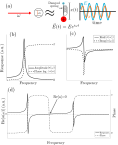
\includegraphics{fig/tuneout/lorentz_model}
		\caption{(a) Illustration of the Lorentz oscillator model of polarizability, wherein the dipole moment of atom in an off-resonant light field is approximated by a periodically driven mass-spring system. The response function (b) has a peak at the resonant frequency $\omega_0$, about which the phase of the response flips from 0 to $\pi$. The spectrum (c) shows that at the zero-crossing of the phase, the steady-state amplitude (real part) of the response is zero but the imaginary part is negative, indicating absorption of energy from the driving force (resonance). A multi-level atom can be approximated by the superposition of such oscillators which give rise to multiple resonances (d). Between the resonances there is also a sign-flip of the phase, coincident with a zero-crossing of the real part. The position of these 'tune-out' points depends on the positions and relative strengths of the resonances.}
		\label{fig:lorentz}
	\end{figure}
	
	Recall from chapter \ref{chap:theory} that an atom in an oscillating electric field experiences an energy shift.
	The magnitude of this shift is proportional to the real part of the dynamic polarizability $\alpha(f)$, a fundamental atomic property determined by the frequency $f$ of the oscillating electric field, the spacing of energy levels, and the strengths of the respective dipole matrix elements.
	This can be illustrated by the classical Lorentz model which approximates the atomic dipole moment by a fixed positive charge plus a negatively-charged particle attached to the `nucleus' by a spring (illustrated in Fig. \ref{fig:lorentz})\footnote{An equivalent model can be constructed using an LC circuit.}.s
	The object of ultimate interest is the equation of motion, which in the Lorentz model is 
	\begin{equation}
		\ddot{x} + \Gamma \dot{x} + \omega_0^2x = -e\vec{E}/m.
	\end{equation}
	Here, $m$ is the mass of the `electron' and the spring has resonant frequency $\omega_0$ and damping rate $\Gamma$, as illustrated in Fig. \ref{fig:lorentz}.
	The general solution for the equation of motion has the form $x(t) = a(\omega)|\vec{E}|e^{i\omega t}$, whose frequency spectrum has a Lorentzian profile,
	\begin{equation}
		a(\omega) = -\frac{e}{m}\frac{1}{(\omega_0^2-\omega^2)+i\Gamma\omega},
	\end{equation}
	where the real part gives the steady-state amplitude of the induced oscillation, and the imaginary part relates to the exchange of energy from the electric field.
	In fact, a real atom possesses many resonances and to first order (in the linear-response regime) the total response is the sum over all resonances, as in $a(\omega) = \sum_i A_i a_i(\omega)$. 
	Thus there generally exist points in the spectrum where the real part of $a(\omega)$ vanishes, which are determined by the resonant frequency and oscillator strength of each possible transition from the current state of the atom.
	
	In the quantum picture a similar correspondence holds: The real part of the polarizability $\alpha(\omega)$ gives the energy shift as a result of a perturbing light beam, and the imaginary part fixes the photon scattering rate  via $\Gamma_{sc} = \textrm{Im}(\alpha)I/(\hbar\varepsilon_0 c)$ in a monochromatic light field with intensity $I$. 
	For a multilevel atom in the state $i$ under the dipole- and rotating-wave approximations \cite{Grimm00} the Stark shift is
	
	\begin{align}
		\Delta E &= -\frac{1}{2\epsilon_0 c}\mathrm{Re}(\alpha(f))\\
		 	&= -\sum_{j\neq i}\frac{|\bra{j}\hat{\mu}\cdot\mathrm{\textbf{E}}\ket{i}|^2}{E_i-E_j}
			% &= -\sum_{j\neq i}\frac{F_{ij}?}{E_i-E_j},		 	
		\label{eqn:dipole_shift}
	\end{align}
	
	\noindent where the $E_i$ are the unperturbed energies, and $\hat{\mu}\cdot\mathrm{\textbf{E}}$ is the dipole interaction energy.
	In the quantum-mechanical framework the strength of these resonances is characterized by the oscillator strengths $f_{ij}$, which are proportional to the (squared) matrix elements $|\bra{j}\hat{\mu}\cdot\mathrm{\textbf{E}}\ket{i}|^2$.
	A ‘tune-out’ frequency (labeled $f_\mathrm{TO}$) occurs between transition frequencies at the point where the contributions to the dynamic polarizability\footnote{For brevity, and as we are concerned solely with the real part of the polarizability, we will simply use the notation $\alpha(f)$ to refer to the \emph{real} part of the polarizability.} $\alpha(f)$ from transitions below that frequency are balanced by those above it (i.e. $\alpha(f)=0$) \cite{LeBlanc07}. 
	This balance point, illustrated in Fig. \ref{fig:he_polz} is therefore fixed by the strength (via the numerator in the RHS of Eqn \ref{eqn:dipole_shift}) and frequency (via the denominator) of every transition in the atomic spectrum and thus provides a precise constraint on the ratio of transition dipole matrix elements. 
	The frequency-dependend polarizability for \mhe~is also shown in Fig. \ref{fig:he_polz} spanning just under 2.5 octaves.

	\begin{figure} 
		\centering
		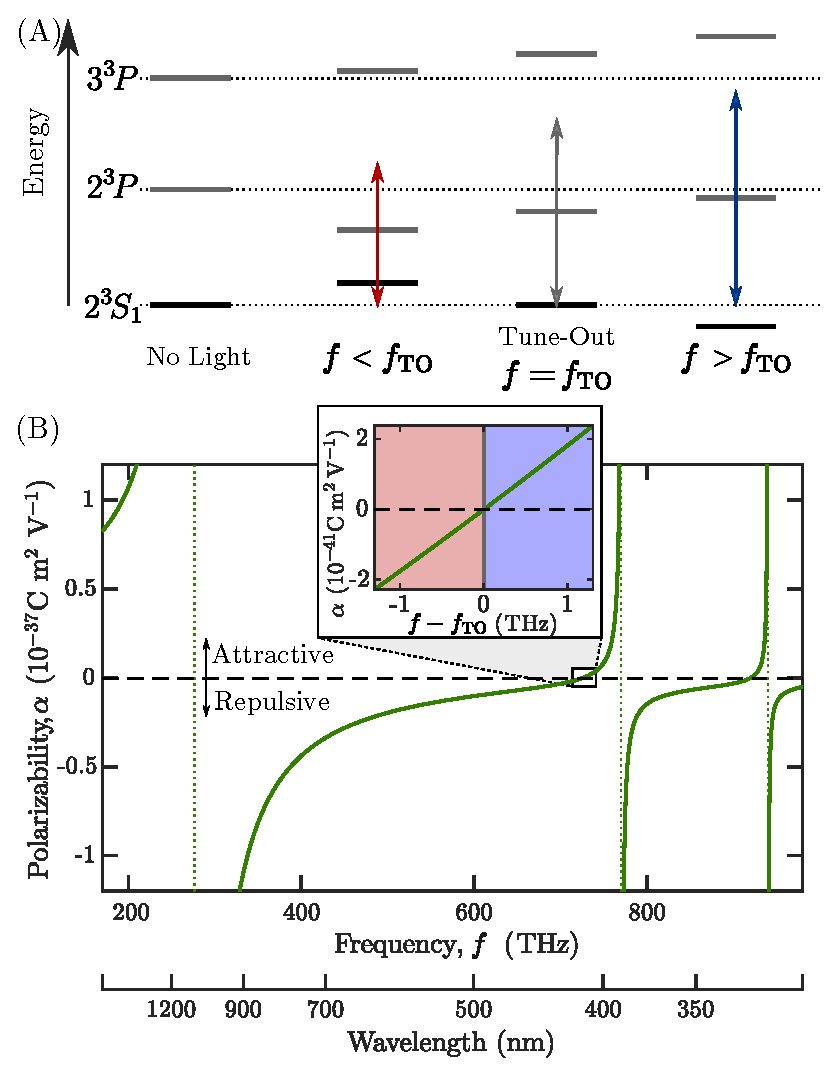
\includegraphics[width=\textwidth]{fig/tuneout/composite_polz_fig}
		\caption{Tune-out in atomic helium:
		(A) Atomic energy level shift of the dominant state (manifolds) about the tune-out.  When an optical field of frequency $f$ (arrows) is applied to the atom the individual
		levels shift dependent on the difference between $f$ and the transition frequency. At the tune-out frequency $f_{\mathrm{TO}}$ (middle right), the shifts to the $\MetastableState$ state energy cancel.
		Energy spacing and shifts not to scale.
		(B) Theoretical frequency dependent polarizability of $\MetastableState$ helium, for a constant light polarisation, indicating that the polarizability vanishes near 726~THz, - the tune-out frequency measured in this paper. 
		Vertical dotted lines show, from left to right, the transitions to the  $\TOLowerStateManifold$, $\TOUpperStateManifold$,$4^{3\!}P$ manifolds. Inset shows the approximately linear polarizability with frequency about the tune-out.
		}
		\label{fig:he_polz} 
	\end{figure}



\subsection{Polarizability near $\fto$}
\label{sec:polz_linearization}

	% % in \cite{LeKien13}
	% % [17,18,20] scalar and tensor polz calculated for Sr and [21,22] For Cs motivated by calculation of magic wavelengths
	% % [16] variety of ways to calculate polarizabilities
	% % [17-19] magic wavelengths are those for which both upper and lower states of a transition are shifted by equal amounts 
	% % [23,24] tune-out wavelength searches for alkali-metal atoms
	% % [25] there are three components, scalar tensor and vector
	% % [33] calc sof SVT polz for Rb
	% % [37] imaginary part of polz is related to the scattering rate

	% The time-dependent polarization of an atom in response to a time-varying electric field is governed by the dynamical polarizability \cite{LeKien13}.
	
	The atomic polarizability has a complex profile, as shown in Fig. \ref{fig:he_polz}, but as we are concerned with measurements in a small region around a tune-out point, we can simplify the analysis below by linearizing the polarizability with respect to frequency. This assumption breaks down if one were to make measurements over much wider frequency intervals, and the magnitude of the loss of accuracy is quantified in section \ref{sec:systematic_effects}.
	In the rest of this section, I describe how the tune-out depends on the frequency and polarization of the laser light, and how this allows us to select a single figure of merit for comparison with theoretical clculations.

	Consider the interaction of an atom with a (real-valued) electric field with the form
	\begin{equation}
		\mathbf{E} = \frac{1}{2}\left(\vec{\mathcal{E}}e^{-2\pi i f t}+\vec{\mathcal{E}}^*e^{2\pi i f t}\right),
	\end{equation}
	where $\vec{\mathcal{E}}=\mathcal{E}\hat{\mathbf{u}}$ is the electric field envelope with magnitude $\mathcal{E}$, polarization vector $\mathbf{u}$ (which may be complex), and oscillation frequency $f$.
	Hereafter in this section, we will consider the atomic reference frame defined by a quantization axis $z$. For a far-off-resonant light field, the Stark shift will be small compared with the fine-structure level splitting. 
	In this case, and working in the dipole appoximation \cite{LeKien13}, the interaction energy between the atomic dipole $\mathbf{d}$ and the light field is captured by the operator
	\begin{equation}
		\Delta E_\mathrm{Stark} = -\frac{1}{2}\left(\mathcal{E}\mathbf{u}\cdot\mathbf{d}e^{-2\pi i f t} - \mathcal{E}^*\mathbf{u}^*\cdot\mathbf{d}e^{2\pi i f t}\right),
	\end{equation}
	which, after a lengthy derivation \cite{LeKien13} can be written as
	\begin{align}
		\Delta E_\mathrm{Stark} &= -\frac{1}{2\epsilon_0 c} \mathrm{Re}(\alpha(f)) I
	\end{align}
	where $I= \frac{\epsilon_0 c}{2} |E|^2$ is the electric field intensity and
	\begin{equation}
		\alpha(f) = \alpha^S + C\alpha^V \frac{m_J}{2J} + D\alpha^T\frac{3m{_J}^{2}-J(J+1)}{2J(2J-1)}
		\label{eqn:full_polz}
	\end{equation}
	% note I = c \epsilon_0 |E|^2/2 so the first line is just Re(a)E^2/4
	is the frequency-dependent polarizability for an atom in a state with total angular momentum $J$ (and a $z$-component of $m_J$).  
	The frequency-dependent scalar, vector, and tensor polarizabilities are $\alpha^S$, $\alpha^V$, and $\alpha^T$, respectively, and the coefficients $C=2\mathrm{Im}(\mb{u}_{x}^{*}\mb{u}_{y})$ and $D= 3|\mb{u}_z|^2-1$ depend on the polarization vector $\mathbf{u}$. More will be said about the polarization effects in section \ref{sec:polz_dep}, but for now let us return to the frequency-dependent effects.
	From the preceding equation \ref{eqn:full_polz} one then obtains the polarizability for the $2\triplet S_1(m_J=1)$ state:
	\begin{equation}
		 \alpha(f) = \alpha^S(f) + \frac{1}{2}\left(C\alpha^V(f)  + D\alpha^T(f)\right).
		 \label{eqn:master_polz}
	\end{equation}
	% in this eqn, D = 3 |u_z|^2 -1, opposite to the Le Kien convention
	Expanding the preceding equation about some frequency $f_0$ near $\fto$ we and truncating the Taylor expansion we have
	\begin{align}
		 \alpha(f)  \approx & \alpha^S(f_0) + (f-f_0)\frac{d\alpha^S}{df}\Bigr|_{f=f_0} \\
		 &+ \frac{C}{2}\left(\alpha^V(f_0) + (f-f_0)\frac{d\alpha^V}{df}\Bigr|_{f=f_0} \right)\\
		 & +\frac{D}{2}\left(\alpha^T(f_0) + (f-f_0)\frac{d\alpha^T}{df}\Bigr|_{f=f_0} \right) + \cdots
	\end{align}
	It is expected on theoretical grounds that the vector and tensor polarizabilities are nearly constant over the scan ranges we use in this experiment (and we can check this experimentally - indeed we do find that the gradient of the fits $\propto d\alpha /d f$ is independent on the polarization, thus only the $\propto d\alpha^S /d f$ is significant).	Hence, we can drop the respective derivative terms and arrive at

	\begin{align}
		 \alpha(f)  \approx & \alpha^S(f_0) + \frac{d\alpha^S}{df}\Bigr|_{f=f_0} (f-f_0) + \frac{C}{2}\alpha^V(f_0) + \frac{D}{2}\alpha^T(f_0).
		 \label{eqn:polz_taylor}
	\end{align}
	The condition that $\alpha(\fto)=0$ implies
	\begin{align}
		 \frac{d\alpha^S}{df}\Bigr|_{f=f_0} (\fto-f_0) \approx & -\alpha^S(f_0) - \frac{C}{2}\alpha^V(f_0) - \frac{D}{2}\alpha^T(f_0).
	\end{align}
	We can simplify this result by setting $f_0$ to be the tune-out for the scalar polarizability, i.e. $f_0=\fto^S$ s.t. $\alpha^S(\fto^S)=0$, thus arriving at
	\begin{align}
		 \fto \approx & \fto^S - \frac{C}{2}\beta^V(\fto^S) - \frac{D}{2}\beta^T(\fto^S)
		 \label{eqn:redpolz}
	\end{align}
	\begin{equation}
		\beta^X(f) = \alpha^X(f)\left(\frac{d\alpha^S}{df}\Bigr|_{f=f_0}\right)^{-1}
	\end{equation}
	for $X\in\{V,T\}$.

	The main conclusions of the preceding calculations is that the polarizability is well-approximated by the linearized equation (\ref{eqn:polz_taylor}) for experimentally relevant detunings from the tune-out. The change in polarizability with respect to frequency is dominated by the scalar term $\alpha^S(f)$, but the zero-crossing of the total polarizability $\alpha(f)$ is modified by the polarization-dependent terms ($\frac{C}{2}\beta^V(\fto^S)$ and $\frac{D}{2}\beta^T(\fto^S)$). Therefore, the tune-out frequency depends on the polarization of the laser beam (Eqn. (\ref{eqn:redpolz})), and so we need to establish some terminology to relate the beam parameters to the atomic dipole response. As we will see below, this also permits us to define a single measurable quantity that can be compared directly with theory.

	% Tang: When A cos \theta_k is adjusted from -1 to 1 the TO shifts by 0.4-6 pm 
	% We must specify a quantity in order to make an unambiguous comparison with theoretical calculations, and thus far we have only manifold of possible values subject to the constraint that $\mathbf{u}^*\cdot\mathbf{u}=1$.
	% We can do this in such a way that eliminates the large effect of $\alpha^V$ by exploiting the interrelationship between the components of $\mathbf{u}$.

	% could continue by expanding about \fto^S and then finding a more general condition for \fto in terms of \fto^S and the other alphas, more like in paper. But what is the point here, really? Time to work thorugh the polz at last...





\subsection{Polarization dependence of the tune-out}
	\label{sec:polz_dep}
	We can now turn attention back to the $C$ and $D$ coefficients. These are most easily expressed in terms of the polarization vector $\mathbf{u}$ and have the form
	\begin{align}
		C &= 2\mathrm{Im}(\mathbf{u}_{x'}^*\mathbf{u}_{y'}),\\
		D &= 3|\mathbf{u}_{z'}|^2-1,
	\end{align}
	where each element can be decomposed as $\mathbf{u}_{x'} = u_{x'} e^{i\phi_{x'}}$, etc.
	The dashed coordinate labels correspond to the atomic reference frame defined by $\hat{z'} = \mathbf{B}/|\mathbf{B}|$, see Fig. \ref{fig:polz_figure}.
	However, the magnetic field vector at the interrogation zone is not necessarily perfectly aligned with the laser beam axis and thus we need a means to translate between different coordinate systems.
	Therefore, before we return to the tune-out equation \ref{eqn:redpolz} we take a short detour here to build up the language necessary to discuss the role of polarization in determining the tune-out frequency.
	The bulk of this section is devoted to introducing the detailed theory of light polarization. For an operational reading of this section, one can consult Fig. \ref{fig:polz_figure} and skip ahead to section \ref{ssec:connection_to_experiment}

% \subsubsection{Theory of light polarization}
	

	\begin{figure}
	\centering
	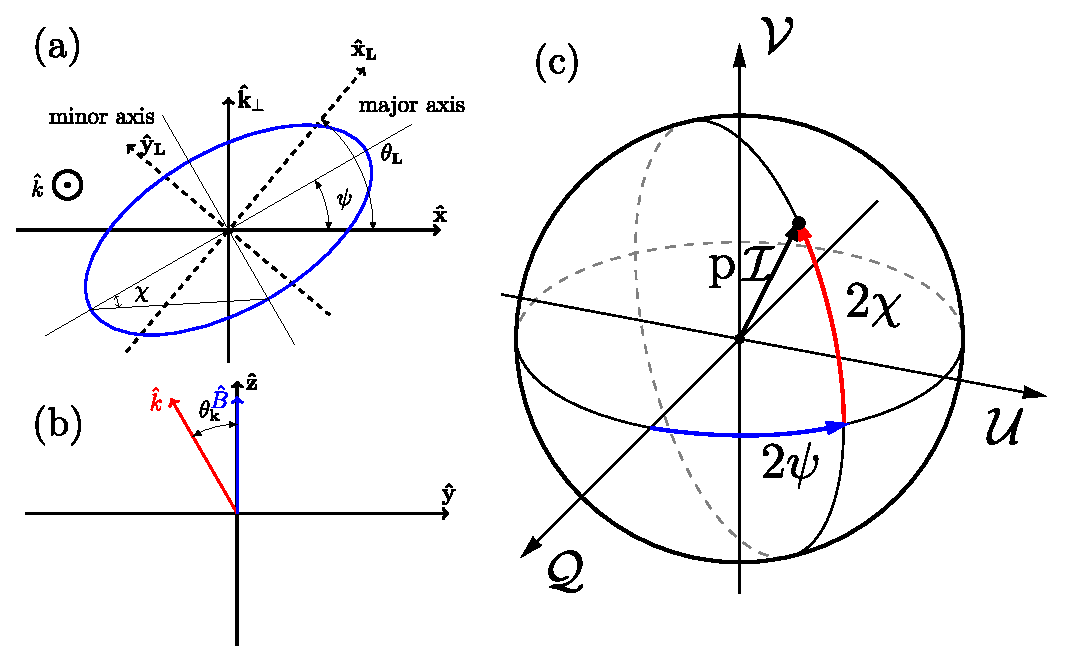
\includegraphics[width=\textwidth]{fig/tuneout/polz_diags}
	\caption{Aspects of light polarization in relation to the experiment. The polarization vector traces out an ellipse in the plane transverse to the light wavevector $\mathbf{k}$, depicted in (a). The ellipse traced in the plane normal to the propagation vector $\hat{k}$ is characterized by the angle $\psi$ between the major axis and the horizontal, and the angle $\chi$ determines the ellipticity (i.e. degree of circular polarization). The lab frame ($\hat{x}_L$) is rotated by an angle $\theta_L$ with respect to the atomic frame.  The light wave-vector is also potentially misaligned with the magnetic field vector, which defines the quantization axis of atomic angular momentum, as shown in (b). Such a possible misalignment factors into the transformation through the angle $\theta_k$. The polarization state can be treated as a real vector on the Poincar\'{e} sphere (c), on which the relationships between the elliptical angles are marked ($\chi$, the degree of circular polarization, gives the elevation angle in red. $\psi$ gives the polar angle, shown in blue). The position of the Stokes vector specifies a polarization state in terms of the Stokes parameters ($\st{Q,U,V}$), as described in the text. For example, circularly polarized light has an angle $\chi=\pi/4$ and thus an elevation angle $\pi/2$, thus living on the `north' or `south' poles of the Poincar\'{e} sphere ($|\st{V}|=1$). 
	}
	\label{fig:polz_figure}
	\end{figure}

	\subsubsection{Theory of polarized light}

	A monochromatic electric field takes on a classical state as
	\begin{equation}
		\vec{E}(\mathbf{r},t) = \mathcal{E}(\mathbf{r},t)\hat{\mathbf{u}}(\mathbf{r}),
		\label{eqn:lightfield}
	\end{equation}
	where $\hat{\mathbf{u}}$ is the unit polarization vector. The electric field propagates in the direction of the Poynting vector $\mathbf{S} = \mathbf{E}\times\mathbf{B}$, and hence we have $\hat{\mathbf{u}}\perp\mathbf{S}$ and $\hat{\mathbf{u}}\perp\vec{k}$, where $\vec{k}$ is the wave-vector of the light. Therefore, if we fix $z'$ as the propagation direction (i.e. along the beam axis, which we will relate the dashed coordinates to the lab frame shortly) then we can write the electric field in the coordinates $(x',y',z')$ as 
	\begin{equation}
		\vec{E}(\mathbf{r},t) = \begin{bmatrix}u_{x'}e^{i\phi_{x'}}\\
												u_{y'}e^{i\phi_{y'}}\\
												0
												\end{bmatrix}e^{i(kz'-2\pi f t)}.
	\end{equation}
	One can then consider the first two components, also known as the \emph{Jones vector} which captures the amplitude and relative phases in the $x'$ and $y'$ direction.
	We can write the Jones vector as a scalar multiplied by a unit-length vector $\hat{\mathbf{j}}$, and following a rotation by an angle $-\phi_x'$ we obtain
	\begin{align}
		\mathbf{j} &= |E|~\hat{\mathbf{j}}e^{-2\pi i f t},~\mathrm{where}\\
				\hat{\mathbf{j}}&= \begin{bmatrix}u_{x'}\\
								u_{y'}e^{i(\phi_{y'}-\phi_{x'})}\end{bmatrix}
	\end{align}
	and $u_{x'}={E_{x'}}/{|E|}$ (and similarly for $y'$).
	As the polarization vector precesses in time (as per the $t$-dependence in Eqn. \ref{eqn:lightfield}) it traces out a locus in the $x',y'$ plane normal to $\vec{k}$.
	For purely-polarized monochromatic light this locus is an ellipse, or rather the Lissajous figure whose $x'$ ($y'$) amplitude is given by $u_{x'}$ ($u_{y'}$) and the relative phase is $\phi_{y'}-\phi_{x'}$.
	Thus we have, for example, circularly polarized light when $u_{x'}=u_{y'}$ and $\phi_{y'}-\phi_{x'}=\pi/2$, or $\hat{\mathbf{j}} = (1,i)/\sqrt{2}$. On the other hand, if $\phi_{y'}-\phi_{x'}=0$ the light is linearly polarized along the axis given by $(u_{x'},u_{v'})$. 
	Up to a factor corresponding to the global phase, the Jones vector notation can be used to express the common polarization states of light in the following forms:

	
	\begin{minipage}{0.5\textwidth}
	\begin{align*}
	\mathbf{h} &= \begin{bmatrix}1\\0\end{bmatrix} \\
	\mathbf{d} =& \frac{1}{\sqrt{2}}\begin{bmatrix}1\\1\end{bmatrix} \\
	\mathbf{l} =& \frac{1}{\sqrt{2}}\begin{bmatrix}1\\i\end{bmatrix} 
	\end{align*}
	\end{minipage}
	\begin{minipage}{0.5\textwidth}
	\begin{align*}
		\mathbf{v} &= \begin{bmatrix}0\\1\end{bmatrix}\\
		\mathbf{a} =& \frac{1}{\sqrt{2}}\begin{bmatrix}1\\-1\end{bmatrix}\\
		\mathbf{r} =& \frac{1}{\sqrt{2}}\begin{bmatrix}1\\-i\end{bmatrix},
	\end{align*}
	\end{minipage}
	\hfill

	% \begin{tabular}{c c}
	% 	\centering
	% 	$\mathbf{h} = \begin{bmatrix}1\\0\end{bmatrix}$ & $\mathbf{v} = \begin{bmatrix}0\\1\end{bmatrix}$\\
	% 	&\\
	% 	$\mathbf{d} = \frac{1}{\sqrt{2}}\begin{bmatrix}1\\1\end{bmatrix}$ & $\mathbf{a} = \frac{1}{\sqrt{2}}\begin{bmatrix}1\\-1\end{bmatrix}$\\
	% 	&\\
	% 	$\mathbf{l} = \frac{1}{\sqrt{2}}\begin{bmatrix}1\\i\end{bmatrix}$ & $\mathbf{r} = \frac{1}{\sqrt{2}}\begin{bmatrix}1\\-i\end{bmatrix}$,
	% \end{tabular}
	% \end{table*}
	\noindent where the row-wise pairs correspond to the orthogonal pairs of horizontal/vertical, diagonal/antidiagonal, and left/right-circular polarization, respectively.
	Indeed any $\hat{\mathbf{j}}$ can be written as a linear combination of any row-wise pair of these vectors with complex coefficients.
	We can take a moment to notice that $\hat{\mathbf{j}}$ is a two-dimensional complex vector of length 1, and thus inhabits the same space as any two-level quantum system - i.e. a qubit.
	The coherence matrix\footnote{Elsewhere called the coherency matrix.} can thus be defined through the outer product
	\begin{align}
		\mathbf{\chi} &= \mathbf{j}^\dagger\otimes\mathbf{j} \\
		 &= \st{I} \begin{bmatrix} u_{x'}^2 & u_{x'} u_{y'} e^{-i(\phi_{x'}-\phi_{y'})} \\ u_{x'} u_{y'} e^{i(\phi_{x'}-\phi_{y'})} & u_{y'}^2\end{bmatrix},
	\end{align}
	where $I=|E|^2$ (which, up to some physical constants, is the intensity of the light field), and the off-diagonal elements are called the \emph{coherences}. 
	The outer product also maps the conventional polarization basis vectors to their respective matrix forms:

	\begin{minipage}{0.5\textwidth}
	\vspace{0pt}
	\begin{align*}
		{H} &= \begin{bmatrix}1&0\\0&0\end{bmatrix} \\
		{D} =& \frac{1}{{2}}\begin{bmatrix}1&1\\1&1\end{bmatrix}\\
		{L} =& \frac{1}{{2}}\begin{bmatrix}1&-i\\i&1\end{bmatrix}
	\end{align*}
	\end{minipage}
	\begin{minipage}{0.5\textwidth}
	\vspace{0pt}
	\begin{align*}
		{V} &= \begin{bmatrix}0&0\\0&1\end{bmatrix}\\
		{A} =& \frac{1}{{2}}\begin{bmatrix}1&-1\\-1&1\end{bmatrix}\\
		{R} =& \frac{1}{{2}}\begin{bmatrix}1&i\\-i&1\end{bmatrix}.
	\end{align*}
	\end{minipage}
	% \hfill

	% \begin{table*}[!h]
	% \centering
	% \begin{tabular}{c c}
	% 	${H} = \begin{bmatrix}1&0\\0&0\end{bmatrix}$ 					& ${V} = \begin{bmatrix}0&0\\0&1\end{bmatrix}$\\
	% 	&\\
	% 	${D} = \frac{1}{{2}}\begin{bmatrix}1&1\\1&1\end{bmatrix}$ &$ {A} = \frac{1}{{2}}\begin{bmatrix}1&-1\\-1&1\end{bmatrix}$\\
	% 	&\\
	% 	${L} = \frac{1}{{2}}\begin{bmatrix}1&-i\\i&1\end{bmatrix}$ & ${R} = \frac{1}{{2}}\begin{bmatrix}1&i\\-i&1\end{bmatrix}$.
	% \end{tabular}
	% \end{table*}
	
	The coherence matrix contains the full polarization information for a classical light-field and can be written in the Pauli basis as $\mathbf{\chi} = \sum_{i=0}^3 a_i\sigma^{i}$, where

	% \begin{table*}[!h]
	% \centering
	% \begin{tabular}
		% $\sigma_0 = \begin{bmatrix}1&0\\0&1\end{bmatrix}$, & $\sigma_1 = \begin{bmatrix}0&1\\1&0\end{bmatrix}$,\\
		% $\sigma_3 = \begin{bmatrix}0&-i\\i&0\end{bmatrix}$, and & $\sigma_3 = \begin{bmatrix}1&0\\0&-1\end{bmatrix}$.
	% \end{tabular}
	% \end{table*}

	\begin{minipage}{0.5\textwidth}
	\vspace{0pt}
	\begin{align*}
	\sigma_0 &= \begin{bmatrix}1&0\\0&1\end{bmatrix}\\
	\sigma_2 &= \begin{bmatrix}0&1\\1&0\end{bmatrix}
	\end{align*}
	\end{minipage}
	\hfill
	\begin{minipage}{0.5\textwidth}
	\vspace{0pt}
	\begin{align*}
		\sigma_1 &= \begin{bmatrix}1&0\\0&-1\end{bmatrix}\\
		\sigma_3 &= \begin{bmatrix}0&-i\\i&0\end{bmatrix}.
	\end{align*}
	\end{minipage}
	% \hfill


	% \begin{table*}[!h]
	% \centering
	% \begin{tabular}{c c}
	% 	$\sigma_0 = \begin{bmatrix}1&0\\0&1\end{bmatrix}$ 					&  $\sigma_1 = \begin{bmatrix}1&0\\0&-1\end{bmatrix}$\\
	% 	&\\
	% 	$\sigma_2 = \begin{bmatrix}0&1\\1&0\end{bmatrix}$ & $\sigma_3 = \begin{bmatrix}0&-i\\i&0\end{bmatrix}.$ \\
	% \end{tabular}
	% \end{table*}
	thus the coherence matrix can generally be written in the form $\chi = \frac{p\st{I}}{2}\left(\mb{1} + p\mathbf{s}\cdot\mathbf{\sigma}\right)$ where $\mathbf{s}=(\st{Q},\st{U},\st{V})\in\mathbb{R}^3$ and $|\mathbf{s}|=1$, analogous to the expression of a qubit state as a Bloch vector, where $\mb{1}=\sigma_0$ is the identity matrix\footnote{Note that the subscript indices differ from the Bloch sphere convention, opting instead for the convention consistent with the Stokes parameters.}.
	Note also that, as for the density matrix in the context of quantum states, the coherence matrix can be used to deal with statistical mixtures of polarization states. In this case, the purity $p\leq1$ can be introduced as a multiplying factor of the length of the (unit) Stokes vector $\mb{s}$. Fully incoherent light has $p=0$ and corresponds to the zero vector in the Stokes picture. Partially coherent light, for example an equal statistical mixture of $\mb{a}$ and $\mb{r}$, has a nonzero Stokes vector ($\frac{1}{2}(\mb{a}+\mb{r})=\frac{1}{2\sqrt{2}}(2,-(1+i))$) which lies inside the Poincar\'{e} sphere, while purely-polarized light lives on the surface of the sphere.
	
	By convention, the full form of the Stokes vector is $\mathbf{S} = (p\st{I},\st{Q},\st{U},\st{V})$ where $I$ corresponds to the beam intensity and the latter three components are the degrees of linear polarization ($\st{Q}$=$\pm$1 for horizontally and vertically polarized light), (anti-) diagonal polarization (accordingly, $\st{U}=\pm1$), and circular polarization (where we pick $\st{V}=\pm1$ for left- and right-circular polarization in the frame defined by the beam axis). Hereafter, we consider the case of purely-polarized light with $p=1$.
	Further, in the coherence matrix picture, the degree of polarization along vector $P$ (expressible as a linear combination of $\{H,V,D,A,R,L\}$) is given by the inner product Tr($\chi P$), as the algebra of the inner product is preserved under the linear action of the tensor product. 
	Completing the analogy, the pairs of orthogonal polarization are related by the transformation $\mathbf{s}\rightarrow-\mathbf{s}$ (just as orthogonal states of a qubit are at antipodal points on the Bloch sphere).
	
	The Stokes vector is illustrated on the Poincar\'{e} sphere, in relation to the polarization ellipse, in Fig. \ref{fig:polz_figure}.
	Notice that in taking the outer product, the factor $e^{\pm2\pi i f t}$ has vanished - the coherence matrix, just as for the density matrix, discards the global phase information by construction. 
	This can be a problem in applications concerning the coherent nature of laser light, wherein the Jones calculus is preferred for its preservation of phase information.
	However, in our case we are concerned with the time-averaged behaviour of the atom-light interaction (c.f. section \ref{sec:atoms_and_light}) and so this loss is not critical.
	For our treatment, we are considering purely polarized light in the experimental context of applying wave-plates after the output from a polarizing beamsplitter, and can do without this parameter.


\subsubsection*{Connection to experiment}
	\label{ssec:connection_to_experiment}

	A full definition of the Stokes parameters in terms of the unit electric field polarization vector $\mb{u}$ the $x',y'$ basis is:
	\begin{align}
	    \mathcal{I} &= |\mathbf{u}_{x'}|^2 + |\mathbf{u}_{y'}|^2 \\ 
	    \mathcal{Q} &= |\mathbf{u}_{x'}|^2 - |\mathbf{u}_{y'}|^2 \\
	    \mathcal{U} &= 2 \text{Re} \left(\mathbf{u}_{x'} \mathbf{u}_{y'}^*\right) \\
	    \mathcal{V} &= -2 \text{Im}\left(\mathbf{u}_{x'} \mathbf{u}_{y'}^*\right)
	\end{align}
	Which allows an expression in the form
	\begin{equation}
		\mathbf{S} = A \mathcal{J},
	\end{equation}
	where
	\begin{equation}
		A=\begin{bmatrix}
		 1 & 0 & 0 & 1 \\
		 1 & 0 & 0 & -1 \\
		 0 & 1 & 1 & 0 \\
		 0 & -i & i & 0 \\
		\end{bmatrix}
	\end{equation}
	and 
	\begin{align}
		\mathcal{J} &= \mathbf{j}^*\otimes\mathbf{j}\\
					&= (u_{x'}^2,u_{x'}u_{y'}e^{-i(\phi_{y'}-\phi_{x'})},u_{x'}u_{y'}e^{i(\phi_{y'}-\phi_{x'})},u_{y'}^2)^\mathrm{T},
	\end{align}
	Therefore the electric field components can be recovered, up to a global phase, via
	\begin{align}
		 \mathcal{J} &= A^{-1} \mathbf{S}\\
					 &= \frac{1}{2}\begin{bmatrix} 
					 				\st{I}+\st{Q}\\\st{U}+i\st{V}\\\st{U}-i\st{V}\\\st{I}-\st{Q}
								 	\end{bmatrix}.
	\end{align}
	thus the electric field components and their relative phase can be recovered through
	\begin{equation}
		 u_{x'} = \sqrt{\frac{\st{I}+\st{Q}}{2}},~u_{y'} = \sqrt{\frac{\st{I}-\st{Q}}{2}},~\phi_{y'}-\phi_{x'} = \mathrm{arctan}(\st{V}/\sqrt{1-\st{V}^2}),
	\end{equation}
	noting that, as expected, we are unable to retrieve the global phase information. For purely-polarized light, whose amplitude is obtained by $\sqrt{\st{I}}$, the real three-dimensional Stokes vector only contains enough parameters to specify the Jones vector. 
	However, we introduce the Stokes parameters for their utility in capturing the polarization-dependence of the atomic polarizability.


	We can now examine the $C$ and $D$ coefficients directly.
	Writing out the coefficient $C=2\mathrm{Im}(u_{x}^*u_y)$ we see it can be obtained by 
	\begin{equation}
	C=2\mathrm{Im}(u_{x}^*u_y) = -\mathrm{Tr}(\sigma_3\chi) = -\st{V}.
	\end{equation}
	That is, it gives the fourth stokes parameter, the degree of (right-) circular polarization in the atomic frame (indeed this follows directly from the definition of $\st{V}$).
	The $D$ coefficient can be seen to depend on the length of the polarization vector along the $z$ axis in the atomic frame, and can be shown \cite{Henson22} to depend on the second Stokes parameter $Q$ through
	\begin{equation}
		D = \frac{3}{2}\sin^2(\theta_k)(1+\st{Q}) - 1,
	\end{equation}
	where $\theta_k$ is the angle between the magnetic field pointing $\hat{b}$ and $\mathbf{k}$.
	The linearized tune-out equation thus reads
	\begin{align}
		 \fto = & \fto^S + \frac{\st{V}}{2}\beta^V - \frac{1}{2}\beta^T \left(\frac{3}{2}\sin^2(\theta_k)(1+\st{Q}) - 1\right)
		 \label{eqn:fto_stokes_eqn}
	\end{align}
	in terms of the Stokes parameters in the atomic reference frame. 

	% From which it follows that, in the case of purely-polarized light, one can write
	% \begin{equation}
	% 	\mathbf{j} = \frac{1}{\sqrt{2}}j (\iota + Q\mathbf{h}+V\mathbf{d}+V\mathbf{l}),
	% \end{equation}
	% where $\iota = (1,1)^\mathrm{T}$. 



\subsubsection{Magic wavelengths}
	% \rev{Similarly, `magic' wavelengths (where the light shift of a \emph{transition}, rather than a \emph{level}, cancels) have yielded absolute and relative determinations of DMEs \cite{Herold12,Leonard15}. However, calculations of these wavelengths are not currently competitive in accuracy with experiments \cite{Jasmeet17}, even for helium \cite{Zhang21}, whereas the tune-out wavelength of interest here is amenable to such a comparison.}
	It bears noting that tune-out points are associated with \emph{states} of the atom, where the stark shift $\Delta E_\mathrm{S} =0$.
	A distinct but related concept is `magic wavelengths' which are associated with \emph{transitions} between states and are defined by the point where the differential dynamic polarizability (or differential stark shift) vanishes: $\Delta E_\mathrm{S,U}-\Delta E_\mathrm{S,L} = 0$. 
	Magic wavelengths have attracted a great deal of interest for their utility in constructing optical lattice clocks \cite{Takamoto05,Derevianko11}, decoupling the clock transition frequency from the intensity of the trapping beams.
	% A major technical issue in atom- and ion-based frequency references is the calculation of the Stark shift due to black-body radiation from the vacuum chamber containing the test system \cite{Fasano21}.
	% Precision measurements of magic wavelengths constrain models of the polarizability over large spectral ranges and thus serve to characterize and help suppress black-body shifts in these systems \cite{Chanu20,Fasano21}.			
	% While magic wavelengths are presented by Nature to the scientist, it is also possible to emulate the effect of a magic wavelength by using an additional laser to counteract the Stark shift from a trapping or probe beam \cite{Hilton19}.
	% Recent progress has also overcome the higher-order effects beyond the electric dipole (namely the magnetic dipole, electric quadrupole, and hyperpolarizability effects) by precisely tuning the magic-wavelength trap to a `magic intensity' and achieving a Stark-shift cancellation to the $10^{-19}$  level in a Strontium latttice clock \cite{Ushijima18}.
	% Precision frequency measurements using neutral atoms (and ions \cite{Chanu20}) in optical lattices continue to provide constraints on possible variations in fundamental constants across space and time \cite{Uzan03,Blatt08,Huntemann14} and have been identified as compact detectors for gravitational waves \cite{Kolkowitz16} and dark matter candidates \cite{Derevianko14}.
	% Further, matter-wave guides built using magic wavelengths provide advantages for atom-interferometric gradiometry of gravitational and electromagnetic fields \cite{Akatsuka17}
	% Finally, magic (and indeed tune-out) wavelengths have recently been reported for ultracold diatomic molecules, thus extending the suite of control options available at the frontier of ultracold matter sciences \cite{Bause20}.


	Magic wavelengths are, of course, also of interest for their potential use in tests of basic atomic structure theory.
	However, most magic wavelength measurements to date have been made using heavy elements like strontium \cite{BilickiThesis}, barium \cite{Chanu20}, mercury \cite{Yi11}, rubidium \cite{Herold12}, and cesium \cite{Yoon19}, whose complex internal structure restricts the accuracy with which these wavelengths can be predicted.
	For instance, while current predictions of magic wavelengths in heavy elements are yet to reach parts-per-million precision, calculations for helium are already at this level \cite{Wu18,Zhang21_magic}.
	
	Highly precise measurements of magic wavelengths have been used to determine transition matrix elements in rubidium to a relative accuracy better than $10^{-3}$ \cite{Herold12}.
	For comparison, tune-out measurements in rubidium have yielded the ratio of oscillator strengths (rather than their absolute values) with accuracy at the $10^{-4}$ level \cite{Leonard15}.
	
	While the contribution of QED effects are included for helium magic wavelengths, their contribution is generally smaller than the theoretical uncertainty associated with the individual energy levels and thus are not yet ready for comparison with experiments.
	However, a very recent work identified the 1335 nm magic wavelength as a candidate for tests of atomic structure theory due to its sensitivity to the finite nuclear mass, and relativistic and QED effects \cite{Zhang21_magic} (contributing to the wavelength at the level of 232, 247, and 21 ppm respectively).
	A measurement of this wavelength to 0.01 nm precision (fractional error $\sim10^{-5}$) would suffice to check the predicted QED contributions.
	
	Indeed, magic wavelengths have already found use in tests of QED with helium, albeit through their role as dipole traps for precision measurements of forbidden transition energies \cite{Rengelink18}.
	A further application to helium was recently proposed wherein one would use a 1265 nm magic wavelength optical trap while another 934 nm magic wavelength beam provides the first of two photons for dichroic excitation of the forbidden $2\triplet S_1\rightarrow 3\triplet S_1$ transition near 427.7 nm \cite{Thomas20, Zhang21_forbidden}.
	This would reduce the effect of the main systematic uncertainty (the AC Stark shift) from 5 MHz to below 100 kHz.

	%% From Li-Yan's document (helium.pdf); the dynamic polarizability is $\alpha_1(\omega) = \sum_n \frac{f_{0n}}{\Delta E_{0n}^2 - \omega^2}$ in terms of all those oscillator strengths


	% \subsection{Other TO measurements}
	% 	\begin{itemize}
	% 	\item \todo{Read these past measurements}
	% 	\end{itemize}
	
	
	
	% As a test of QED, a tune-out frequency is advantageous because it is a null measurement, which does not require calibration of the light intensity or a measurement of excitation probability. These factors have previously limited the precision of direct transition strength measurements \cite{Boloufa09,Vogt07,Thomas20}. In comparison, previous tune-out measurements have been successful in measuring QED effects \cite{Leonard15,Holmgren12,Schmidt16,Herold12,Henson15}.
	% 2015 safranova theoretical identification of TO wavelengths in Strontium, check their accuracy
	% 	Ref for extracting transition rates
	% 	https://journals.aps.org/pra/abstract/10.1103/PhysRevA.92.040501

	% 2011 TOs for alkali metals, v early theory work
	% 	https://journals.aps.org/pra/abstract/10.1103/PhysRevA.84.043401
	% 2013 Cheng calculations of TOs for alkali-earth metals
	% 	https://journals.aps.org/pra/abstract/10.1103/PhysRevA.88.022511
	% 2013 Jiang prediction of TO wavelengths for potassium
	% 	https://journals.aps.org/pra/abstract/10.1103/PhysRevA.87.032518
	% 2016 Wang tune-outs in R, high precision measurements to 790.018187(193) and 790.032602(193) nm
	% 	Agree with theory (Leonard 15)
	% 	https://journals.aps.org/pra/abstract/10.1103/PhysRevA.94.052510
	% 2016 Schmidt 790nm tuneout in Rb by KD scattering of a BEC
	% 	790.01858(23) nm with sub-pm accuracy
	% 	https://journals.aps.org/pra/abstract/10.1103/PhysRevA.93.022507
	% 2016 Dammalapati calcs of magic and TOs for francium
	% 	https://journals.aps.org/pra/abstract/10.1103/PhysRevA.93.043407
	% 2017 Trubko Potassium TO 768.9701(4) nm using atom interferometry
	% 	 Ratio of oscillator strenghts inferred 2.066(11), ratio of line strenghts 1.9977(11)
	% 	https://journals.aps.org/pra/abstract/10.1103/PhysRevA.95.052507
	% 2017 Kao Dysprosium TO measurement, reported to the percent level, using kapitza-dirac diffraction
	% 	https://www.osapublishing.org/oe/fulltext.cfm?uri=oe-25-4-3411&id=359890 
	% 2017 Leonard high precision Rb tune-out measurement
	% 	erratum: Actual value = 790.032 326(32) nm, matrix element ratio 1.992 17(3)
	% 	theoretical value 790.0315(7) (after correction)

	% 2018 Tang predictions of Thallium TO and magics
	% 	https://journals.aps.org/pra/abstract/10.1103/PhysRevA.98.062511
	% 2019 Copenhaver 7Li tune-out measurement with atom interferometry
	% 	 3329.5(1.4) MHz for the tensor-shifted tune out  with σ± light polarization and 3310.6(4.9) MHz with scalar polz
	% 	 good ref for distinction between terms
	% 	https://journals.aps.org/pra/abstract/10.1103/PhysRevA.100.063603
	% 2020 Decamps 671nm TO for 7Li by atom interferometry
	% 	Can be corrected (via tensor terms) to agree with Copenhaver et al
	% 	https://journals.aps.org/pra/abstract/10.1103/PhysRevA.101.033614
	% 2020 Jian tune-out wavelength for 133Cs
	% 	Calculation - check precision, and note that tensor part is very very small in this case
	% 	https://journals.aps.org/pra/abstract/10.1103/PhysRevA.102.042823
	% 2021 Jiang tuneouts for Ba+ ions
	% 	Precision looks quite good
	% 	Sensitive to QED?
	% 	https://journals.aps.org/pra/abstract/10.1103/PhysRevA.103.032803
\subsection*{QED prediction of the tune-out point}
\label{sec:to_theory}
	% theory work
	Following the first prediction \cite{Mitroy13} and measurement  of the metastable helium  tune-out near 413 nm \cite{Henson15}, a vigorous campaign of theoretical studies \cite{Zhang16,ManaloThesis,Drake19,Zhang19, Pachucki19} has reduced the uncertainty in the predicted frequency, which previously limited comparison with experiment. In parallel with work at ANU, our collaborators\footnote{Namely Gordon Drake and Li-Yan Tang, with assistance from Aaron Bondy and Yong-Hui Zhang.} improved on the state-of-the-art calculation \cite{Zhang19} of the tune-out frequency.

	These calculations were performed using the non-relativistic QED method (nr-QED) and improve the precision by an order of magnitude (compared to the previous prediction \cite{Mitroy13}) with a total uncertainty at the level of 9 MHz (relative error $1.2\times10^{-8}$) . 
	The results are presented in Table~\ref{tab:theory} with a summary explanation here. A more detailed description is in the full manuscript \cite{Henson22}.
	
	\begin{table}[t]
	\centering
	%\vbox{\hsize 5.2in \noindent
	% \begin{ruledtabular}
	\begin{tabular}{l r r}
	\hline\hline
	Quantity    &Value (MHz) & Uncertainty (MHz) \\
	\hline
	\multicolumn{3}{c}{\textbf{Nonrelativistic and Relativistic terms}} \\
	Nonrelativistic (NR) & 725\,645\,115& 2       \\
	NR + relativistic scalar $(\alpha^{\rm S})$    & 725\,742\,216&6   \\
	Relativistic tensor $(-\frac12\alpha^{\rm T})$ &   1\,755& \\
	\hline
	Total non-QED        & 725\,743\,950&6     \\
	\hline
	\multicolumn{3}{c}{\textbf{QED terms}} \\
	QED $\alpha^3$       &       -7\,298& 1       \\
	QED $\alpha^4$       &          -127& 6       \\
	\hline
	Total QED            &         -7\,425& 8     \\
	\hline
	Retardation          &          -477 &        \\
	Nuclear size         &             5&          \\
	\hline
	Grand total          & 725\,736\,053& 9       \\
	Experiment           & 725\,736\,700& 260 \\
	\hline
	Difference           &          -647& 260\\
	\hline\hline
	\end{tabular}\\
	\caption{\label{tab:theory}Summary of theoretical contributions to the helium $\TO$ manifold tune-out frequency near 725.7 THz.}
	\label{tab:theory}
	% \end{ruledtabular}
	\end{table}

	The entries from nonrelativistic, relativistic, and QED contributions are not strictly additive because changing one effect, such as the relativistic correction, changes the tune-out frequency at which the other effects are evaluated.  Thus the first entry is the nonrelativistic tune-out frequency with finite nuclear mass effects included.  The next entry is the scalar part of the relativistic correction arising from the higher terms in the Breit interaction.  The entry from the spin-spin interaction (1755~MHz) is entirely responsible for the tensor part of the tune-out frequency (excluding the Schwinger radiative correction term $\alpha/\pi$).  These terms determine the nonrelativistic and relativistic part of the tune-out frequency.  The remaining terms are small enough that they can be added linearly.  The leading QED correction of order $\alpha^3$ ($-7298(6)$ MHz) includes the anomalous magnetic moment correction (8 MHz).  The terms of order $\alpha^4$ include only the radiative corrections.  The dominant source of uncertainty is thus the remaining nonradiative terms not included in the calculation, but which were previously computed for the $2^3S_1$ state energy \cite{Pachucki06}.  The remaining terms are the retardation correction of $-477$ MHz and a finite nuclear size correction.
	 % by accounting for finite nuclear size and mass, relativistic, QED, negative energy states, and finite wavelength retardation effects \cite{Drake19, Pachucki19,Henson22}. 
	% The interaction of an isolated atom with a freely propagating laser field is regarded as a zero in the coherent Rayleigh scattering cross section, rather than as a zero in the dynamic polarizability as is the case for an atom in an optical lattice. The two formulations are identical in lowest order, but not when retardation (finite wavelength) effects are taken into account. For convenience I will continue to use the $\alpha_(\omega)$ notation to denote a zero in the Rayleigh scattering cross section.

	% The nr-QED method considers the nonrelativistic Schr\"odinger equation and includes terms for the Breit interaction by perturbation theory \cite{BetheSalpeter,Piszczatowski15,Puchalski16,Puchalski20}.  The dynamic polarizability is expressed to second order in the interaction with a monochromatic oscillating electromagnetic field, and contributions from relativistic and QED effects enter through an additional perturbation.  
	% The included relativistic corrections are the spin-independent terms, the orbit-orbit interaction, the spin-dependent spin-spin interaction, and the Darwin term (see \cite{Henson22} for definitions and calculation of the aforementioned terms).
	% QED corrections are included in the form of effective operators up to fourth order in $\alpha$ \cite{Yerokhin10}, including the Araki-Sucher terms \cite{Araki57,Sucher58} ($\alpha^3$) and radiative QED terms ($\alpha^4$). The remaining nonradiative terms, amounting to about 5\% of the contributions from the radiative terms for the $2^3S_1$ state \cite{Piszczatowski15,Pachucki06}, result in an uncertainty of about 6MHz and are considered the dominant uncertainty.	A significant contribution of the theoretical work is the inclusion of retardation corrections recently derived by Pachucki and Puchalski \cite{Pachucki19,Drake19}.  These additions represent a reformulation of the problem as a zero in the coherent Rayleigh scattering amplitude for an atom in free space, instead of a zero in the frequency-dependent polarizability for an atom in an optical lattice \cite{Pachucki19,Drake19}. 






\section{Measurement technique}
\label{sec:trap_freq_measure}
	


	\begin{figure}
	\begin{minipage}{0.5\textwidth}
	\vspace{0pt}
	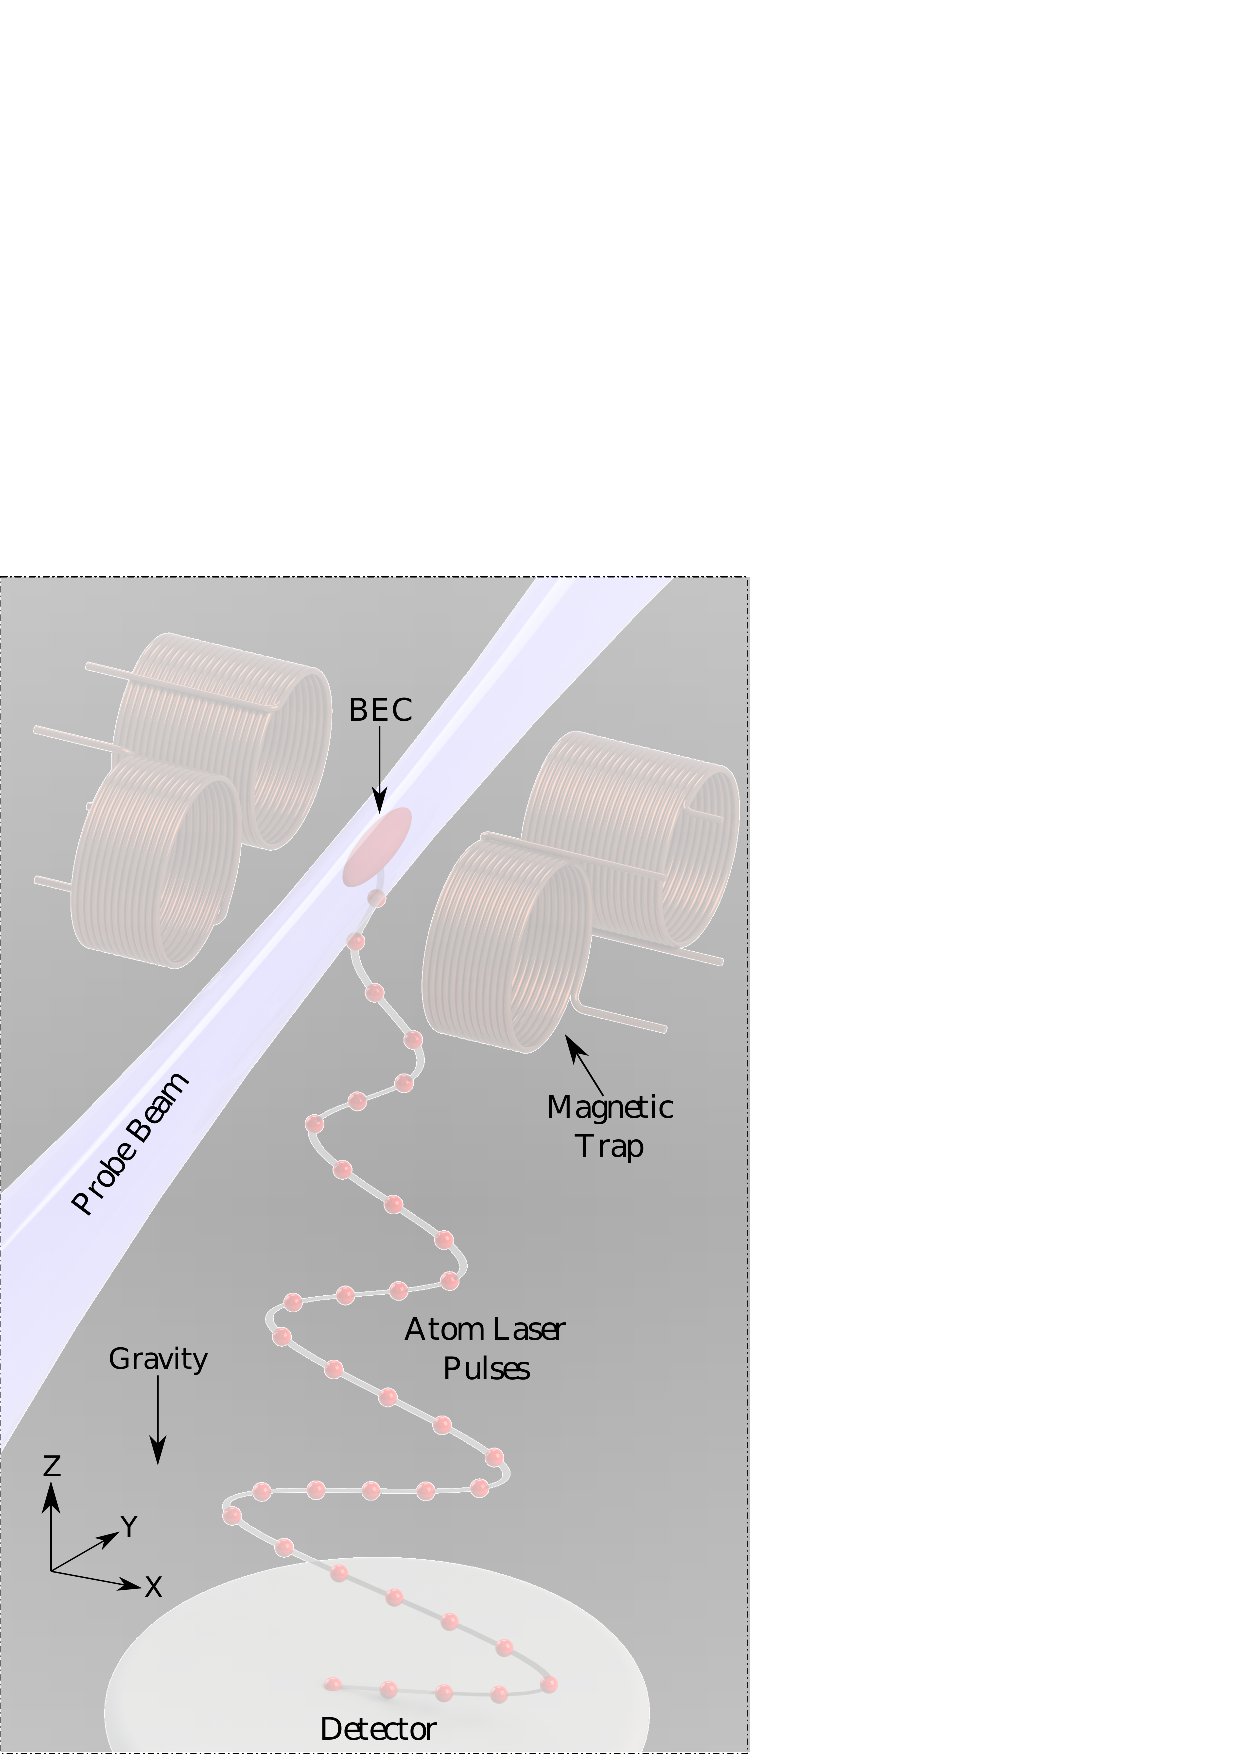
\includegraphics[width=\textwidth]{fig/tuneout/exp_schematic.png}
	\end{minipage}
	\hfill
	\begin{minipage}{0.5\textwidth}
	\vspace{0pt}
	\caption{
	Schematic of the physical system used to determine the tune-out frequency as a function of laser frequency. A magnetically trapped BEC of metastable helium atoms is illuminated with a probe laser beam with an adjustable (optical) frequency. The probe beam is aligned with the weak axis of the trap and oscillations are induced in the BEC centre of mass. The oscillation direction is horizontal and transverse to the laser beam, aligned with the axes of the BiQUIC coils.  A sequence of atom laser pulses (red spheres) is outcoupled from the BEC to sample the oscillation. The oscillation frequency is reconstructed by the anti-aliasing procedure described in section \ref{sec:trap_freq_meas}
	The lab-frame coordinate axes show the oscillation direction $y$, transverse to the beam axis $x$.
	}
	\label{fig:exp_schematic} 
	\end{minipage}
	\end{figure}

	Having defined a tune-out, we now turn our attention to the means we employed to determine the 413 nm tune-out using our apparatus. 
	This section provides a physical description of the measurement technique and establishes the important roles played by the frequency and polarization of the probe beam.
	To determine a tune-out point is essentially to measure the frequency where the optical dipole potential  vanishes.
	In our measurement, we quantified the shift in the oscillation frequency of a harmonically trapped BEC when the magnetic trap was overlapped with a power-stabilized probe laser beam (see Fig. \ref{fig:exp_schematic} and Section \ref{sec:spec_laser}). 
	This is in contrast to previous works (eg. \cite{Rengelink18}) wherein magic-wavelength optical traps were used in conjunction with a resonant probe beam. 
	The main motivations for the use of a magnetic trap are that it permits the pulsed outcoupling method, enabling the highly accurate trap frequency determinations which underpin this measurement. Furthermore, the magnetic field is easily configured to be extremely harmonic at length scales much larger than the BEC or its in-trap motion.

	The position-dependent potential energy in this hybrid trap is the sum of both the harmonic magnetic potential and a Gaussian optical potential,
	\begin{equation}
		U_\mathrm{net} = U_{\mathrm{trap}} + U_\mathrm{dip},
	\end{equation}
	where the magnetic trapping potential takes the form
	\begin{equation}
		U_\mathrm{trap} = \frac{m}{2}\left(\omega_{x}^{2}x^2+\omega_{y}^{2}y^2+\omega_{z}^{2}z^2 \right)
	\end{equation}
	where the $\omega_i$ terms are the oscillator frequencies of the harmonic magnetic trap, and the dipole potential is given in general by  \cite{Grimm00}
	\begin{align}
	    U_{\mathrm{dip}}=-\frac{1}{2 \epsilon_{0} c} \operatorname{Re}(\alpha) I(\rvec),
	\end{align}
	where $I(\rvec)$ is the local intensity of the electric field, $c$ is the speed of light and $\epsilon_0$ is the permittivity of free space.
	For a Gaussian beam which is aligned with the weak ($x$) axis of the trap and focuses $P$ watts of power to a spot size $w_0$, the intensity profile is 
	\begin{equation}
	    I_{\mathrm{dip}} =
	        \frac{2 P}{\pi w_0^2} \left(\frac{w_0}{w(x)}\right)^2 \exp\left( -\frac{1}{2} \frac{(y^2+z^2)}{w(x)^2} \right)
	 \end{equation}
	 where $w(x) = w_0\sqrt{1+(x/x_R)}$ is the waist size at a position $x$ along the beam axis and $x_R$ is the Rayleigh length. 
	 In the small-amplitude oscillation limit we can consider the total potential to be harmonic and retain only the terms up to second order in a Taylor expansion. If we further assume that the trapped BEC oscillates in the $y$ direction only then we can write the potential along the direction of motion as
	 \begin{equation}
	 U_\mathrm{net} \approx -\frac{\mathrm{Re}(\alpha)  P}{\pi 
   c {w_0}^2 \epsilon} + \left(\frac{2 \mathrm{Re}(\alpha)  P}{\pi  c {w_0}^4 \epsilon }+\frac{m {\omega_y}^2}{2}\right) y^2
	 \end{equation}
	 when evaluated about $x=z=0$.
	 Noting that the restoring force for a harmonic oscillator is given by $F_y = -\partial_y U_\mathrm{net} = -k_\mathrm{net} y$, we can identify the perturbed trapping frequency via the spring constant $k_y$:
	 \begin{align}
	 	\Omega_\mathrm{net} &= \frac{1}{2\pi}\sqrt{\frac{k_\mathrm{net}}{m}}\\
	 	&= \frac{1}{2\pi}\sqrt{{\omega_y}^2+\frac{4 P \mathrm{Re}(\alpha)}{\pi m c \epsilon w_{0}^4}}
	 \end{align}
	wherein we can identify the trap and probe frequency contributions by setting $P=0$ and $\omega_y=0$, respectively. 
	We thus obtain 
	\begin{equation}
		\Omega_\mathrm{probe} = \frac{1}{2\pi}\sqrt{\frac{4 \mathrm{Re}(\alpha)  P}{\pi m c \epsilon w_{0}^4}}
		\label{eqn:omega_probe}
	\end{equation}
	and have the relation
	\begin{align}
		\Omega_\mathrm{net}^2 &= \Omega_\mathrm{trap}^2 + \Omega_\mathrm{probe}^2\\
		&= \Omega_\mathrm{trap}^2 + \frac{4P}{\pi m c \epsilon w_{0}^4}\mathrm{Re}(\alpha)
		\label{eq:delta_omega_squared}
	\end{align}
	which shows that the squared shift in trapping frequency $\Omega_\mathrm{probe}^2 = \Omega_\mathrm{net}^2 - \Omega_\mathrm{trap}^2$ is linear in the probe power and the polarizability.
	Note the $\Omega$ terms have units 1/time - the trapping frequencies $\omega_i$ are angular frequencies with units Rad Hz. Thus, $\Omega_\textrm{trap} = \omega_y/2\pi$.
	
	\begin{figure}
	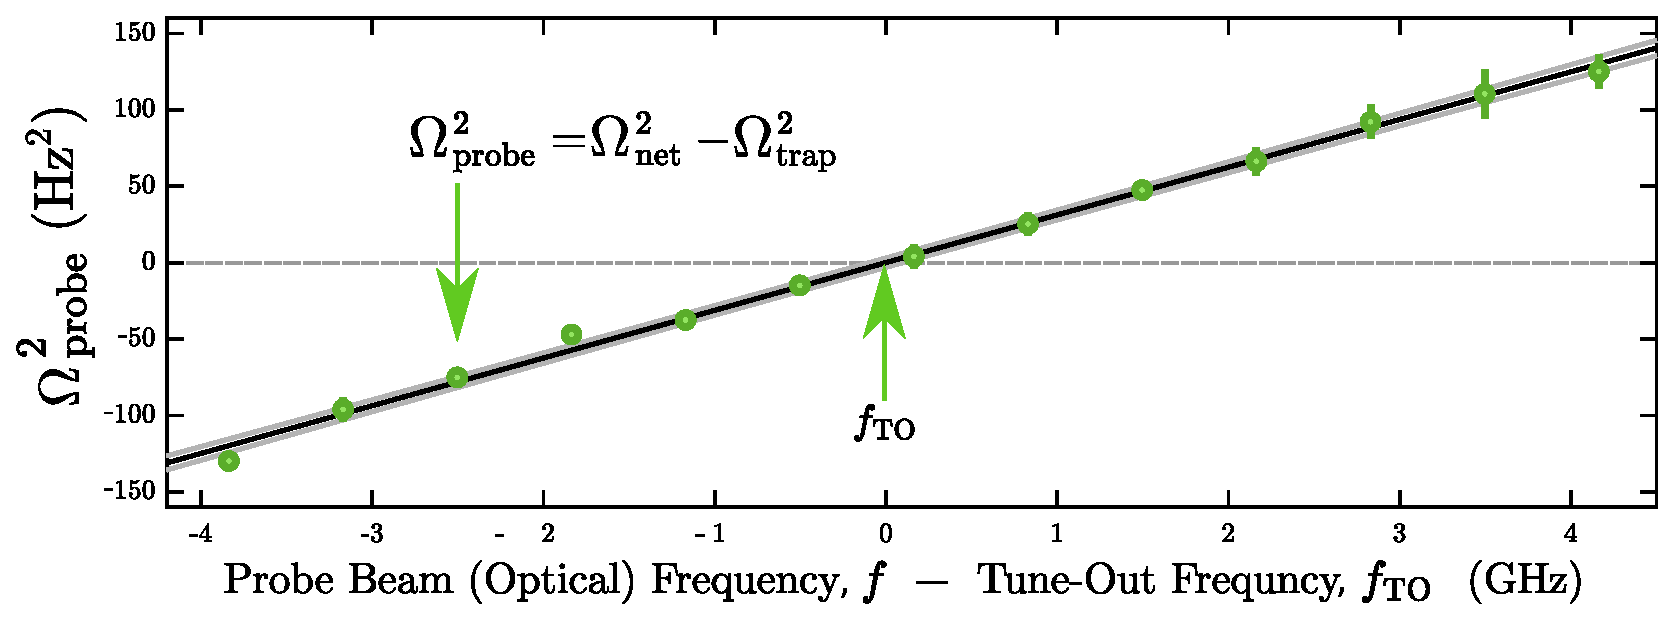
\includegraphics[width=\textwidth]{fig/tuneout/freq_scan}
	\caption{
	Determining the tune-out frequency for fixed polarization. The squared probe beam trap frequency (response) is found by comparison to a measurement of the unperturbed trap frequency. We repeated these measurements over a small frequency interval and extract the tune-out by finding the \textit{x}-intercept of the response. Also shown is the linear fit (black solid line) with light grey lines showing the \(1\sigma\) confidence intervals about the expected value of the mean. All error bars on points represent the standard error in the mean.
	}
	\label{fig:freq_scan} 
	\end{figure}

	An immediate corollary of Eqn. \ref{eq:delta_omega_squared} is that if the probe beam power is stabilized then $\Omega_\mathrm{probe}^2$	is linear solely in $\mathrm{Re}(\alpha)$. 
	It then follows that ascertaining the frequency at which $\Omega_\mathrm{probe}=0$ constitutes a determination of the tune-out point.
	Figure \ref{fig:freq_scan} shows the linear variation of experimentally-determined values of $\Omega_\mathrm{probe}^2$ versus the probe beam frequency $f$, demonstrating that this approximation holds in practise. 
	Indeed, we found that including a quadratic term in a fit to $\Omega_\mathrm{probe}^2(f)$ yielded an estimate of the zero-crossing frequency that was not statistically distinguishable from the zero-crossing estimate obtained from a linear fit.
	Section \ref{sec:implementation} provides more information about the experimental methods we used to obtain these measurements.





\subsection{Experimental implementation}
	\label{sec:implementation}
	We implemented such a hybrid trap using the BiQUIC machine and the tunable laser system described in chapter \ref{chap:apparatus}, especially section \ref{sec:spec_laser}. 
	The beam was tightly focused down to a waist of order 10 $\mu$m at the magnetic trap centre, then aligned with the weak axis of the harmonic magnetic trap as illustrated in Fig. \ref{fig:exp_schematic}.
	The laser system delivers up to 150 mW of power to the vacuum chamber when operating at the wavelengths relevant to this measurement. 
	We then scanned the laser wavelength $\pm4$ GHz about the tune-out in 13 steps ($\sim666.7$ MHz intervals), depicted in Fig. \ref{fig:freq_scan} .	
	This range is chosen in order to minimize the nonlinearities that are present when the optical potential is strong (see the discussion of systematic effects in section \ref{sec:systematic_effects}) while still presenting a sufficient signal-to-noise for interpolation of the linear response.
	
	For a given magnetic or hybrid (magnetic and optical) trap, the trap frequency can be determined by repeatedly sampling the momentum during a single shot using a pulsed atom laser. 
	The trap frequency measurement technique is discussed briefly in the next section, and in more detail in the next chapter (specifically section \ref{sec:n0_cal}). 
	First, I describe the experimental sequence used to realize the test conditions.
	Each measurement began with the production of a BEC of $(6\pm1)\times10^5$ \mhe~atoms\footnote{The variation in atom number reflects the range of atom numbers used in all runs. Generally the atom number in a given data collection run has a standard deviation of no more than 10\% of the mean.} cooled to $\sim80$ nK ($T/T_c\approx 0.1$) to reduce damping via coupling to the thermal part.
	Just prior to the frequency measurement we applied a 50~$\mu$s current pulse to a small coil near the BEC, inducing oscillation in the $y$-axis with initial amplitude (velocity) of $\approx30~\mu$m ($15$ mm/s).
	About 1\% of the atoms in the BEC were outcoupled every 8ms by a 5$\mu$s pulse of RF radiation (resonant with the trap centre at 1.7 MHz), creating a pulsed atom laser.
	The outcoupled atoms are in the $m_J=0$ state which is unaffected by magnetic fields, including the trap, and thereafter freely fall the 852~mm to the MCP-DLD (section \ref{sec:DLD}).
	From the time-of-flight data we reconstruct the initial velocity of each atom.
	The average velocity of atoms in a given pulse is an estimate of the centre-of-mass velocity of the BEC at the time the pulse was applied.
	The in-trap oscillation thus resolves as a variation in the centre-of-mass position on the detector, as shown in Fig. \ref{fig:trap_freq_eg}.
	The underlying trap frequency is then determined by means of the anti-aliasing technique described in the next section and in section \ref{sec:n0_cal}.
	Ultracold clouds below the condensation temperature were used because thermal clouds are more strongly damped in their oscillation, which is the dominant limitation for the precision of the trap frequency measurement described below (see e.g., \cite{Henson22_PAL}). 
	This is a major factor in the improved precision of this measurement over the previous one \cite{Henson15}, thus while thermal clouds can certainly be used, they would compromise the accuracy of the measurement.
	% We gradually increased the RF power during the pulses to maintain a good signal-to-noise ratio for later pulses, which would otherwise be hampered by the geometric decay of the pulse population.
	% A fit using a model of the form $y = A \exp(-t/\tau)\sin(\omega_\mathrm{net}+\phi)$ to 130 samples of the mean velocity (see fig \ref{}) thus determines the trap frequency to within 10~mHz in a single experimental cycle. 

\subsubsection{Measuring the trapping frequency}
	\label{sec:trap_freq_meas}

	The oscillation frequency can be determined by fitting a damped sine wave to the centre-of-mass velocity as a function of time, as shown in Fig. \ref{fig:trap_freq_eg}.
	The sampling rate of the pulsed atom laser is limited by the velocity width of the BEC in the vertical axis (\(\sim40\)~mm/s, which corresponds to a temporal width at the detector of \(\sim\)4~ms) along with the vertical oscillation amplitude. This presents a challenge for measuring the trap frequency as the oscillation is much faster than the sampling rate. 
	Thus the true oscillation frequency is \emph{aliased} to a frequency below the Nyquist frequency of the sampling (with an 8 ms period, the sampling rate is 125~Hz, and the Nyquist frequency is half this again, about 62 Hz).
	It is possible to reconstruct the true trapping frequency using an anti-aliasing technique which I describe in more detail in section \ref{sec:n0_cal}.
	We find that our magnetic trap is extremely stable, with characterisic frequencies of $(\omega_x,\omega_y,\omega_z)= 2\pi\times(55.4(3),426.6(1),428.41(4))$ Hz (where the values in brackets represent the standard deviation all measurements, which is larger than the typical variation within a single run).
	\begin{figure}
	\centering
		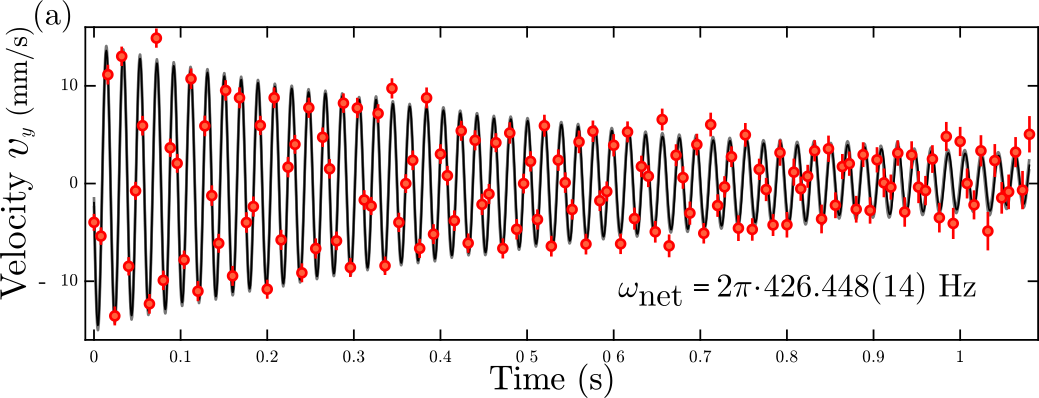
\includegraphics[width=0.8\textwidth]{fig/tuneout/trap_freq_eg}
			\caption{ Determining the trap frequency. The mean velocity of each pulse in the \textit{y}-direction ($v_y$) is used to trace out the oscillation over time (red points) and extract the oscillation frequency with a damped sine wave fit (solid line) for each realization of a BEC. The fitted frequency parameter is used to obtain the underlying trap frequency, as described in the surrounding text. A single experimental realization is shown.}
			\label{fig:trap_freq_eg}
	\end{figure}	
	
	The trap frequency measurement alternates between the combined trap and a purely magnetic trap to account for any drift in the magnetic trapping frequencies. 
	This calibration permits a determination of $\omega_\mathrm{probe}$ in two shots (about 50 seconds). 
	Given a measurement of the frequency $\omega_\mathrm{net}$ of the combined potential, the trap frequency $\omega_\mathrm{trap}$ (at the time of the interrogation) is predicted  by evaluating an interpolated model of the calibration frequency (smoothed by a Gaussian kernel with $\sigma=60$~s).
	This was done to correct for drifts of the magnetic trap frequency and to reduce noise. 
	The calibration data can also be used to obtain an estimate of the error in the trap frequency, which combines (true) trap frequency variation along with measurement error. 
	% We found that the underlying trap frequency had a standard deviation of 30 mHz across the longest data run, and that the overlapping Allan deviation at the 90s timescale (the smallest determinable given the experiment cycle time) was 18 mHz. 
	% These contribute fractional errors of 70 and 43 ppm, respectively.
	
s
		

	% To illustrate how we obtain the trapping frequencies, consider an undamped harmonic oscillator in one dimension. The centre-of-mass momentum $p(t) = A \cos(2\pi f t))$ oscillates at a frequency $f$ Hz, and the centre of mass of a pulse outcoupled at time $t'$ lands on the detector at a position $x'(t+\tau) = p(t')\tau/m$, where $\tau$ is the time of flight of the centre of mass. Sampling the cloud motion with a sampling period T starting at initial time $t_0$ produces a series of pulses whose centres of mass land at $\{x_n = (A\tau/m) \cos(\omega(t_0+nT))\}$. The sampling frequency $f_s=1/T$ determines the \emph{Nyquist frequency} $f_N=f_s/2$, which is the maximum frequency that can be reconstructed unambiguously from such a sampling regime. When $f>f_N$ the signal manifests as a lower-frequency oscillation known as the \emph{alias} of the signal. The aliased frequency $f_a$ is

	% \begin{equation}
	%  f_a =
	%   \begin{cases}
	%    \frac{Z_N f_s}{2} - f & \text{if } Z_N \text{ even} \\
	%    f - \frac{(Z_N-1)f_s}{2}       & \text{if } Z_N \text{ odd},
	%   \end{cases}
	%   \label{eqn:Z_N}
	% \end{equation}
	
	% where $Z_N = \lceil{f/f_N}\rceil$ is the Nyquist zone number, as described in numerous RF engineering references\footnote{Some good tutorials are presented \href{https://www.analog.com/media/en/training-seminars/tutorials/MT-002.pdf}{here} and \href{https://www.taborelec.com/Multi-Nyquist-Zones-Operation-Solution-Note}{here}.}. While it is not possible to determine $Z_N$ for a signal with an unknown (and not necessarily stationary) $f$ from samples taken at a fixed $f_s$, one can vary $f_s$ and determine both $Z_N$ and $f$.
	





% \subsection{


\subsubsection{Measuring polarization}

	% \newcommand{\Tr}[1]{\mathrm{Tr}}
	% The similarity between the Stokes and Bloch pictures extends even further indeed, permitting us to determine the Stokes parameters in the laboratory frame with simple measurements.
	% The action of a polarizing beamsplitter (PBS) introduces another degree of freedom which specifies the optical path.
	% For a $V$-transmitting PBS the (transmitted, reflected) intensities can be written as $\frac{1}{2}$(1+Tr($\sigma_1\chi$),1-Tr($\sigma_1\chi$)).
	We can measure the polarization of the light beam by use of a polarizing beamsplitter (PBS) and quater-wave plate.
	For our measurements we used a rotating Glan-Thompson polarizer with a high extinction ratio $>10^{5}$ in the transmitted component. 
	The calcite crystal in this type of polarizer internally reflects the $p$-polarized component (parallel to the \emph{plane of incidence} spanned by $\hat{k}$ and the normal to the optical surface) at the crystal interface, which leaves the $s$-polarized (parallel to the reflective surface) to exit through the transmitting port.
	That is, when the reflecting surface is vertical in the laboratory, the vertically-polarized component is transmitted, and the horizontally-polarized component is reflected.
	The fraction $p_T$ of optical power transmitted and reflected by the PBS are given by the projections $p_T=\Tr(\mathrm{V}\chi)=\frac{1-\st{Q}}{2}$ and $p_R=\Tr(\mathrm{H}\chi)=\frac{1+\st{Q}}{2}$, respectively. 
	Therefore one has $\st{Q} = \Tr(\sigma_1\chi) = p_R - p_T$. In terms of the absolute powers $P_T$ and $P_R$ measured at the beamsplitter ports, one must normalize by the total power and find 
	\begin{equation}
		p_R - p_T = \frac{P_R-P_T}{P_R+P_T}.
	\end{equation}
	which is commonly known as the \emph{contrast}.
	If one rotates the polarizer relative to the beam\footnote{This is usually much easier than rotating the lab relative to the polarizer.} by an angle $\theta$, this is equivalent to transforming the Stokes vector by matrix multiplication with
	\begin{equation}
		R(\theta) = \begin{bmatrix}
					1 & 0 & 0 & 0 \\
					0 & \cos(2\theta) & \sin(2\theta) & 0 \\
					0 & -\sin(2\theta) & \cos(2\theta) & 0 \\
					0 & 0 & 0 & 1
					\end{bmatrix}.
	\end{equation}
	The framework for considering the action of linear-optical elements by expressing them in such 4$\times$4 matrices which act on the Stokes vector is known as the Mueller calculus. Accordingly, the preceding matrix is (an example of) a Mueller matrix. 
	This allows a quantification of the observation that the maximum contrast occurs when the reflecting port of the polarizer is aligned (or orthogonal) with the major axis of the polarization ellipse.
	Denoting, then, the maximum and minimum transmitted powers, the maximum contrast (also called the \emph{visibility}) is $(P_\textrm{max}-P_\textrm{min})/(P_\textrm{max}+P_\textrm{min})$, where $P_\textrm{max}$ (resp. $P_\textrm{min}$) is the maximum (minimum) power transmitted over all polarizer angles $\theta$, which occurs when $\theta=\theta_\textrm{max}$ (resp. $\theta=\theta_\textrm{min}$). 
	Due to energy conservation considerations we should have $p_\textrm{max} = 1 - p_\textrm{min}$. 
	Further, if the major axis of the ellipse is at some angle $\theta_L$ from the laboratory $x$-axis, then the transmitted power will be minimized when the polarizer angle is at $\theta_L/2$ relative to the horizontal, c.f. the trigonometric terms in $R(\theta)$.
	Therefore we can obtain the laboratory $\st{Q}$ component via 
	\begin{equation}
		\mathcal{Q_{L}} =\frac{P_{\mathrm{max}}-P_{\mathrm{min}}}{P_{\mathrm{max}}+P_{\mathrm{min}}} \cos(2\theta_{\mathrm{min}}).
	\end{equation}
	We see also that the rotation matrix $R(\theta)$ does not mix the linear polarization components with $\st{V}$; the relative phases of the orthogonal oscillations are invariant.
	However, a similar argument to that just given can show that 
	\begin{equation}
		\mathcal{U_{L}} =\frac{P_{\mathrm{max}}-P_{\mathrm{min}}}{P_{\mathrm{max}}+P_{\mathrm{min}}} \sin(2\theta_{\mathrm{min}}),
	\end{equation}
	and so it follows from $|\mathbf{s}|=1$ that
	\begin{equation}
		\mathcal{V_{L}}^2 =\frac{4 P_\textrm{max}P_\textrm{min}}{(P_\textrm{max}P_\textrm{min})^2},
	\end{equation}
	which determines the degree, but not handedness, of the circular polarization in the lab frame.
	However, as we will see in section \ref{sec:fitting}, the sign of $\st{V}$ need not be determined directly as either sign can be made consistent with the tune-out equation within our analytical procedure.


	% In combination with a half- and quarter-wave plate pair, one can determine the polarization state of the light in a process similar to quantum state tomography of the qubit.
	% The general operator for a waveplate whose fast axis makes an angle $\theta$ with the horizontal, and which has a phase difference $\phi$ between the fast and slow axes, has the form
	% \begin{equation}
	% \mathrm{WP}(\theta,\phi)=\begin{bmatrix}
	% 						 1 & 0 & 0 & 0 \\
	% 						 0 & \cos ^2(2 \theta )+\cos (\phi ) \sin ^2(2 \theta ) & \cos (2 \theta ) (1-\cos (\phi )) \sin (2 \theta ) & \sin (2 \theta ) \sin (\phi ) \\
	% 						 0 & \cos (2 \theta ) (1-\cos (\phi )) \sin (2 \theta ) & \cos (\phi ) \cos ^2(2 \theta )+\sin ^2(2 \theta ) & -\cos (2 \theta ) \sin (\phi ) \\
	% 						 0 & -\sin (2 \theta ) \sin (\phi ) & \cos (2 \theta ) \sin (\phi ) & \cos (\phi ) 
	% \end{bmatrix}
	% \end{equation}
	% when acting on the (full) Stokes vector $\st(I,Q,U,V)$. This is an example of a Mueller matrix, which can also be constructed for other linear-optical elements. Note that the action of the operation is purely on the last three dimensions, leaving the purity and intensity unchanged.
	% A half-wave plate has $\phi=\pi/2$ and thus has an action of the form
	
	% \begin{equation}
	% \mathrm{HWP}(\theta)=\begin{bmatrix}
	% 					 1 & 0 & 0 & 0 \\
	% 					 0 & \cos ^2(2 \theta )-\sin ^2(2 \theta ) & 2 \cos (2 \theta ) \sin (2 \theta ) & 0 \\
	% 					 0 & 2 \cos (2 \theta ) \sin (2 \theta ) & \sin ^2(2 \theta )-\cos ^2(2 \theta ) & 0 \\
	% 					 0 & 0 & 0 & -1 
	% \end{bmatrix}
	% \end{equation}

	% while a quarter-wave plate has $\phi=\pi/4$ and thus has a Mueller matrix of the form

	% \begin{equation}
	% 	\mathrm{QWP}(\theta)=\begin{bmatrix}
	% 						 1 & 0 & 0 & 0 \\
	% 						 0 & \cos ^2(2 \theta ) & \cos (2 \theta ) \sin (2 \theta ) & \sin (2 \theta ) \\
	% 						 0 & \cos (2 \theta ) \sin (2 \theta ) & \sin ^2(2 \theta ) & -\cos (2 \theta ) \\
	% 						 0 & -\sin (2 \theta ) & \cos (2 \theta ) & 0.
 % 	\end{bmatrix}
	% \end{equation}
	% Thus the HWP can be seen to rotate the Stokes vector about the $\st{V}$ axis, while the QWP operation generates a more complicated action which mixes all three polarization components.

	% We employ the so-called power ratio technique to determine the probe beam polarization parameters \(\mathcal{V_{L}},\mathcal{Q_{L}}\) in the laboratory basis\footnote{}. The polarization parameters can be obtained by the relations
	% Define the contrast (the relative difference between either output port, also known as the visibility) as
	% \begin{equation}
	% 	p = \frac{p_{\mathrm{max}}-p_{\mathrm{min}}}{p_{\mathrm{max}}+p_{\mathrm{min}}}
	% \end{equation}
	% For a $V$-transmitting PBS the contrast is 1 for $H$, $V$, $D$, and $A$ light, depending on the angle of the polarizer relative to $u_x$.
	% Notice that if the polarizer is fully transmitting when the angle $\theta_
	% Rotating the polarizer 
	% The plane of polarization for linear light (including D and A light) can be determined by using a half-wave plate, which rotates the Jones vector 
	% If the light is in the any of the D, A, L, or R states, Tr($\sigma_1\chi$)=0 and thus the contrast will be zero.

	% \begin{align}
	%      \mathcal{Q_{L}} &=\frac{p_{\mathrm{max}}-p_{\mathrm{min}}}{p_{\mathrm{max}}+p_{\mathrm{min}}} \cos(2\theta_{\mathrm{min}}), \\
	%      |\mathcal{V}_{\mathcal{L}}| &= \frac{2\sqrt{p_{\mathrm{min}}p_{\mathrm{max}}}}{p_{\mathrm{min}}+p_{\mathrm{max}}},
	% \end{align}
	% where \(p_{\mathrm{max}}\) (\(+p_{\mathrm{min}}\)) is the maximum (minimum) power transmitted. The angle $\theta_{\mathrm{min}}$ is the angle (relative to the beam $x$-axis)  of rotation at which the polarizer transmission is minimized. The handedness of the circular component, which fixes the sign of $\mathcal{V_L}$, can be determined using a rotating quarter wave plate technique. 

\subsubsection*{Polarization at the atoms}

	% Ultimately what I want is to make the transformation $S_L \rightarrow E_L \rightarrow E_A \righarrow S_A$; begin with the Stokes parameters in the lab frame. Then, convert to the electric field representation and perform a coordinate transformation; then perform another transformation to the Stokes parameters in the new frame. 


	The transformation of $\mathcal{Q}$ from the laboratory to the atomic reference frame is given by a rotation around the probe beam axis by the angle \(\mathcal{\theta_{L}}\),
	and hence can be written in terms of the lab-measured parameters as
	\begin{equation}
	 \mathcal{Q_{A}} =\frac{P_{\mathrm{max}}-P_{\mathrm{min}}}{P_{\mathrm{max}}+P_{\mathrm{min}}} \cos(2(\mathcal{\theta_{L}}+\theta_{\mathrm{min}})).
	 \label{eqn:q_transform}
	\end{equation}
	This can also be interpreted as the rotation around the beam axis which aligns the laboratory polarizer angle origin with the component of the magnetic field vector which is orthogonal to $\mathbf{k}$. 
	Note that the circular component of the light is unchanged by the coordinate transformation, thus let us denote \(\mathcal{V_{L}}=\mathcal{V_{A}}\) by  \(\mathcal{V}\) hereafter.
	However, the rotation between the coordinate axes in the lab and atom frames mean that the Stokes parameters in the atomic frame are given by their respective projections, quantified in trigonometric coefficients.
	Thus, the final form of the tune-out equation is
	\begin{align}
		 \fto(\st{Q},\st{V}) = & \fto^S + \frac{\st{V}}{2}\cos{\theta_k}\beta^V - \frac{1}{2}\beta^T \left(\frac{3}{2}\sin^2(\theta_k)(1+\st{Q}) - 1\right)
		 \label{eqn:tune_out_eq}
	\end{align}
	where $\st{Q}=\st{Q_A}(\st{Q_L},\theta_L)$ in the atomic frame, as defined in Eqn. \ref{eqn:q_transform}. 
	The tune-out value $\fto(\st{Q}=-1,\st{V}=0)= \fto^S + \frac{1}{2}\beta^T$ is the sole option that eliminates any dependence on $\theta_k$, and we can leave $\theta_L$ as a fit parameter.

\section{Determination of the tune-out frequency}

	We obtain \(f_{\mathrm{TO}}(-1,0)\) through three stages of measurements. 
	First, as described above, we fix the probe beam polarization $(\mathcal{Q_A},\mathcal{V})$ and frequency $f$, and then measure the atomic polarizability via the squared shift of the centre-of-mass oscillation frequency of a BEC in the combined optical dipole and magnetic potentials ($\Omega_\mathrm{probe}^{2}(f)$).
	Second, we take many such measurements while scanning the probe beam frequency and find the optical frequency where the polarizability is zero for this probe beam polarization (i.e. the tune-out frequency \(f_{TO}(\mathcal{Q_A},\mathcal{V})\)) . 
	Finally, we measure $\fto(\mathcal{Q_A},\mathcal{V})$ for many settings of the probe beam polarization and extract \(f_{\mathrm{TO}}(-1,0)\) through the procedure described in this section. 
	

\label{sec:TO_analysis}

\subsection{Exclusion criteria}

	An experiment this complex is susceptible to many potential failure modes, and it is prudent for the experimentalist to mitigate against them.
	To ensure the integrity of the data set used for analysis we complemented the aforementioned control systems with a veto checklist in the data preprocessing pipeline.
	This consisted of a software screening procedure which discarded any measurements where any of the following essential conditions failed to hold. These conditions result in a loss of only one shot per $10^{4}$ across the whole dataset of 43500 shots. 



	\textbf{Single-mode laser:}	On rare occasions we observed that the Ti:S laser would spontaneously run in a mode where multiple optical frequencies were resonant in the cavity and present in the output, a so-called multi-mode regime (strictly a \emph{temporal} multi-mode regime, as distinct from the case where multiple spatial modes are present in the beam profile). This behaviour would cause the wavemeter to provide inaccurate frequency measurements, and also fail to produce the desired test conditions at the interaction zone. We eliminated runs where this happened by recording the output of a scanning Fabry-Perot cavity (Thorlabs SA200-5B). We scanned the cavity over twice its full free-spectral range in a sawtooth manner by scanning the voltage across a piezoelectric actuator, which modulates the cavity length, at frequency of 20 Hz. 
	We recorded the piezo and photodiode voltage during the interrogation and also in a $\sim0.2$~s period before and after.
	The multimode condition was triggered when the separation between peaks detected in the photodiode voltage were less than the free-spectral range, indicating the presence of multiple optical frequencies.
	To detect these peaks we processed the voltage recordings from the photodiode at the output of the cavity using a peak-detection algorithm. The threshold for detection was a peak height that was $1.5\times10^{-3}$ times the peak transmission intensity, which could distinguish spurious (multimode) peaks from electronic noise (all multimode conditions we  observed had peak intensities some orders of magnitude larger than this).

	\textbf{Stable probe power:}		We employ a check on the probe beam power as measured by a photodiode that monitors a sample of the beam just before it enters the experimental chamber, as shown in Fig.~\ref{fig:tunable_laser}. This ensures that the power feedback system is operating at set point in all measurements used in the analysis. Restrictive thresholds are set on the mean ($<0.02$ fractional difference to set point), standard deviation ($<0.05$ of set point) and maximum difference between the mean and the set point ($<0.03$ of set point) of the power during interrogation.

	\textbf{Stable probe frequency:}		The probe beam frequency at each measurement is taken to be the average optical frequency returned by the wavemeter during the interrogation. Shots were rejected if the frequency records in the lock loop's log file had a standard deviation greater than $3$~MHz or a range greater than $5$~MHz. These thresholds were based on our observations of typical locked performance, wherein the wavemeter reading displayed excursions from the mean that were smaller than the aforementioned ranges.

	\textbf{High atom number:}		Shots with very low atom number would lead to inaccurate determinations of the trapping frequency because the damped-sine fit would not be able to fit to many points. We mitigated this by screening out shots with less than $2\times10^{5}$ detected atoms. We found that the choice of threshold introduces a negligible systematic shift in the final tune-out determination, hence we could use shots with a wide range of atom numbers.


	In the end, it is likely that most of the failed shots would have been detected by the outlier-removal step in the fitting procedure, and thus it is plausible that these exclusion rules were of marginal benefit.However, we did not compare the results of running the analysis with and without the exclusion.

\subsection{Regressing the tune-out against polarization}
 \label{sec:fitting}
	
	% In order to make a definitive comparison between experiment and theory we seek a single quantity, but the working above shows that the tune-out is not uniquely defined.
	% Also, we cannot directly measure \(\mathcal{\theta_{L}}\) or $\theta_k$ with sufficient accuracy.
	% Fortunately we can address both of these issues by judiciously choosing the tune-out for a specific polarization state such that the dependence on these parameters vanishes, which I describe in this section. 
	
	We measured the tune-out frequency for 75 (\(\mathcal{Q_{L}},\mathcal{V}\)) pairs, comprising a total of $736$ tune-out measurements.
	We then fit the linearized model (Eq.~(\ref{eqn:tune_out_eq})) to the data, regressing $\fto$ against the measured $\mathcal{Q_{L}}$ and $\mathcal{V}$ values using five free parameters: $f^{S}_{TO}$ (the frequency at which the scalar polarizability $\alpha^S(f)=0$), the angle $\theta_{\mathcal{L}}$ between the lab and atomic reference frames, the angle $\theta_{k}$ between the beam propagation vector $\hat{k}$ and the magnetic field pointing, and the reduced vector- and tensor-polarizabilities $\beta^V$ and $\beta^T$ (see section \ref{sec:polz_linearization}).
	We can then predict a value for $\fto(-1,0)$, despite the lack of precise knowledge of the magnetic field pointing, by evaluating the resulting model at \(\mathcal{Q_{A}}=-1,\mathcal{V}=0\) to find \(f_{\mathrm{TO}}(-1,0)\). 
	The statistical error in the calculated \(f_{\mathrm{TO}}(-1,0)\) is determined with a bootstrapping technique\footnote{In the bootstrap method, one applies an analysis procedure on subsets of the data. The variance of the resulting findings provides an estimate of the sample variance, quantifying the statistical error in the fit to the entire data set. Source code is available at \cite{bryce_bootstrap_error_code}.}. 
	Figure \ref{fig:full_tune_out} displays the $\mathcal{Q_{A}}$ value calculated from the measured $\mathcal{Q_{L}}$ using the fitted $\theta_{\mathcal{L}}$. The measured \(f_{TO}\) is displayed as a function of $\mathcal{Q_{A}}$, $\mathcal{V}$. Figure ~\ref{fig:full_tune_out} also shows the tune-out calculated using polarization measurements taken before and after the vacuum chamber.
	In Fig. \ref{fig:pol_TO}, the measurements are displayed by interpolating the tune-out measurements to the one-dimensional subspaces defined by $\st{V}=0$ (a) and $\st{Q}=0$ (b).
	\begin{figure}
	    \centering
	    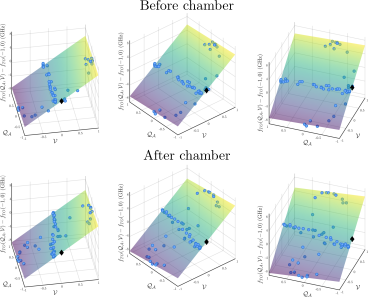
\includegraphics[width=\textwidth]{fig/tuneout/polz_pre_post}
	\caption{Visualizing the fit to $f_{TO}$ as a function of the polarization parameters $\mathcal{Q_{A}}$,\, $\mathcal{V}$  (see Eq.~(\ref{eqn:tune_out_eq})). The top row shows a fit using the polarization data taken before the vacuum chamber. The bottom row uses data taken after the vacuum chamber.  Each tuneout measurement is shown as a blue point. Note that (a-c) and (d-f) show, respectively, different viewing angles on the same data. The black diamond shows the value for \(f_{\mathrm{TO}}(-1,0)\) obtained in each case: \(f_{\mathrm{TO}}(-1,0)=725\, 736\, 810(40)\)~MHz in the top row, and \(f_{\mathrm{TO}}(-1,0)=725\, 736\, 610(40)\)~MHz in the bottom row. The other fit parameters are \(\beta^V \cos(\theta_k)=13240(70)\)~MHz, and \(\beta^T \sin^2(\theta_k)=1140(20)\)~MHz.}
	% top data:\(\beta^V \cos(\theta_k)=13240(70)\)~MHz, and \(\beta^T \sin^2(\theta_k)=1140(20)\)~MHz
	% bottom data: \(\beta^V \cos(\theta_k)=13012(100)\)~MHz, and \(\beta^T \sin^2(\theta_k)=550(100)\)~MHz
	\label{fig:full_tune_out}
	\end{figure}
	
	\begin{figure}
	\centering
	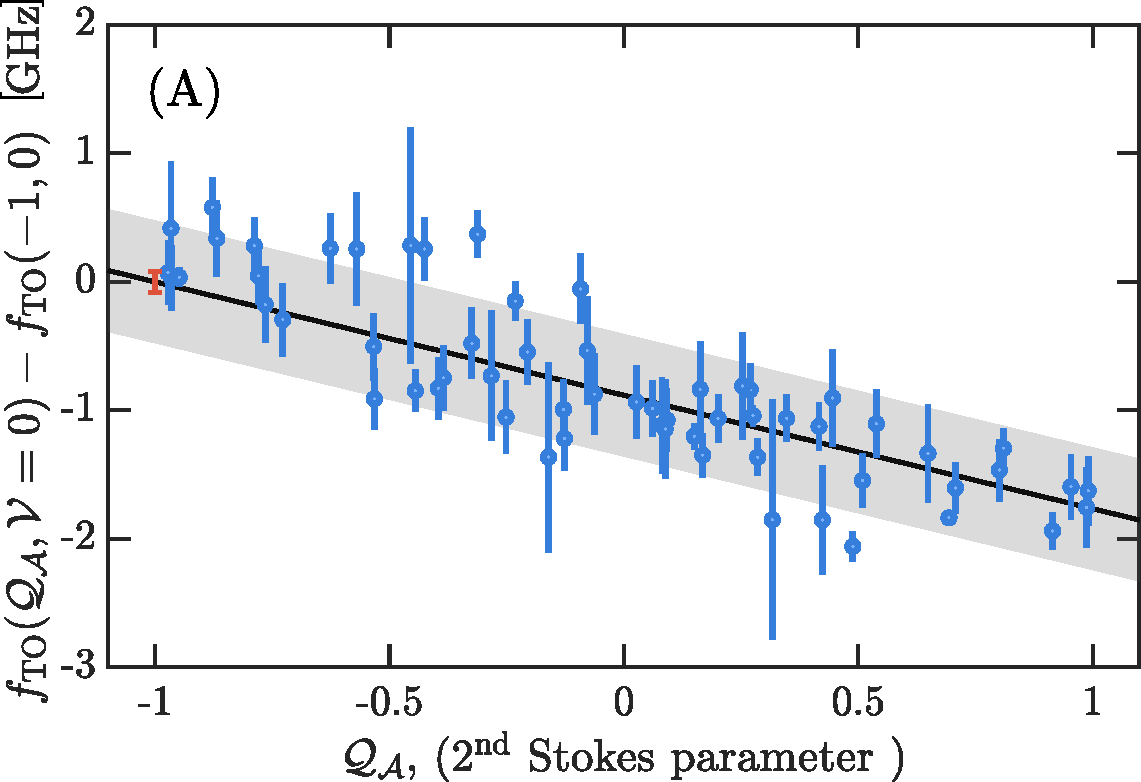
\includegraphics[width=\textwidth]{fig/tuneout/q_dep_1_min.pdf}
	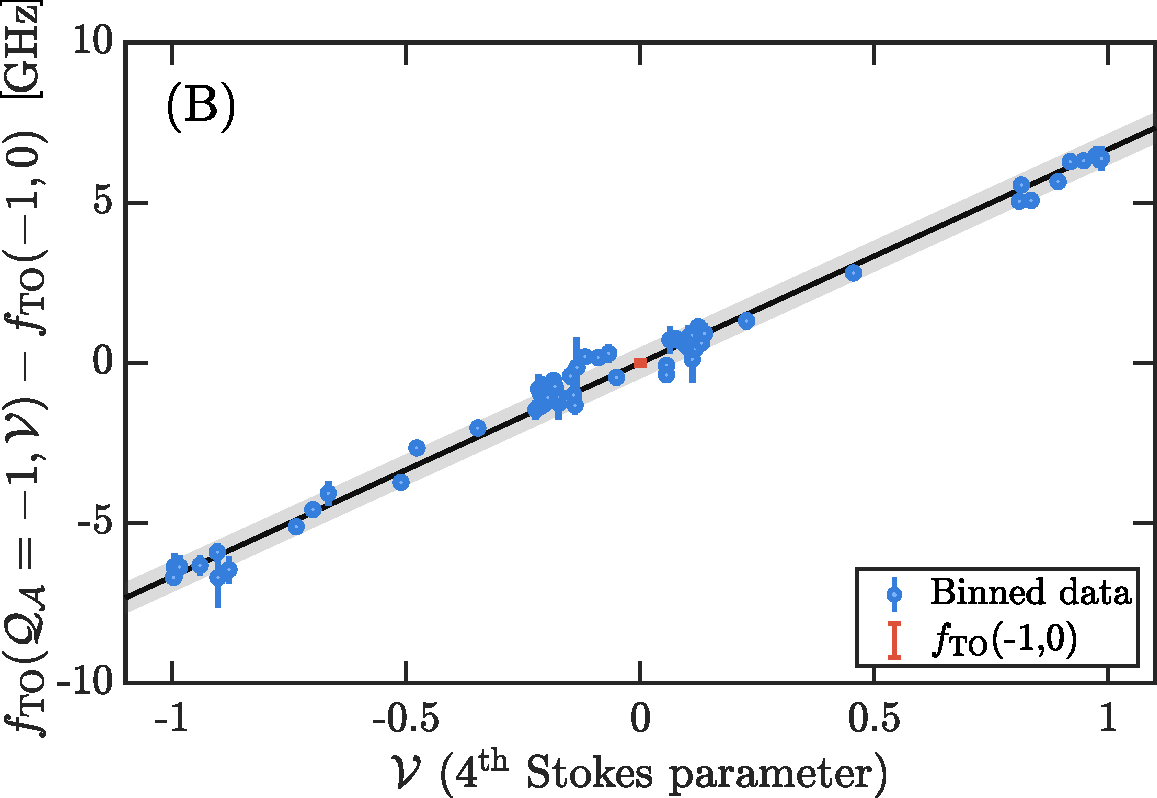
\includegraphics[width=\textwidth]{fig/tuneout/v_dep_1_min.pdf}
	\caption{
	Tune-out dependence on probe beam polarisation.
	% Evaluating the two-dimensional model along the one-dimensional sections defined by $\mathcal{V}=0$ (A) and $\mathcal{Q_{A}}=-1$ (B).
	 In (A), the data points show the $\omega_{TO}$ for each measurement after interpolating to the polarization state  ($\mathcal{Q_{A}},\mathcal{V}=0$). 
	Similarly, (B) shows the interpolation to  ($\mathcal{Q_{A}}=-1,\mathcal{V}$). 
	Error bars on the blue points are the estimated standard error in the mean value for a given polarization. The light-shaded and dark-shaded areas are the $1\sigma$ observation and confidence intervals, respectively. 
	The distinguished point is the predicted $\fto(-1,0)$, with the error bar indicating the (non-simultaneous) confidence interval.
	}
	\label{fig:pol_TO} 
	\end{figure}
	The preceding procedure amounts to finding the plane of best fit for trivariate data (i.e. triples of the form $(\st{Q},\st{V},f_{\mathrm{TO}}(\st{Q,V}))$), which requires only three parameters for complete specification. The use of five free parameters is an over-parametrization of the plane and thus the fit is overdetermined and cannot uniquely fix the fit parameters without additional measurements of at least one such quantity.	
	Further, the fit gives equal agreement between either polarity of \( \beta^T \), compensating by finding a different optimal value for $\theta_L$, and thus preventing a determination of \(f_{\mathrm{TO}}(-1,0)\). 
	To eliminate this issue, we constrain the sign of \( \beta^T \) using measurements and simulations of the magnetic field pointing and theoretical atomic structure calculations, both of which agree with the sign constraint \( \beta^T >0 \).
	We can also see here that the sign of $\st{V}$ is not critical; the cosine term can take on either sign, whereas the sine-squared term will be unchanged by a shift $\theta_k\mapsto\pi-\theta_k$.
	
	The presentation of the fit results in the remainder of this chapter include two distinct quantifications of statistical uncertainty intervals. The \emph{observation interval} quantifies the variance in data that is not explained by the predictor variables $\st{Q}$ and $\st{V}$ (\emph{i.e.} the noise around the mean value). This can also be interpreted as a measure of the expected variance of future observations at a given polarization value. In contrast, \emph{confidence intervals} quantify the uncertainty in the estimates of the model parameters. The  interval for a given confidence level $C$ denotes the range of values wherein a model parameter is expected to lie with a probability of $C$. 
	The confidence interval is similar to the standard error in that additional data can reduce the width of the confidence interval, whereas the observation interval quantifies the systematic variance and does not generally decrease with the addition of more data.
	The stated values for the fit parameters throughout this chapter are generally the 95\% confidence intervals, and when we predict the value of $f_\mathrm{TO}(-1,0)$, the relevant value is the mean value of tune-out measurements at this polarization value, and as such the relevant uncertainty interval is the confidence interval. The 1$\sigma$ observation interval ($C\approx 0.68$) is used to illustrate the variance of the data.

	The validity of the observation interval can be quantified by the reduced chi-squared ($\chi^2$) statistic, defined as follows.
	Given a model with input predictor- and outcome-data tuples $(x_i,y_i)$, the residuals are the difference $r_i=\hat{y}_i - y_i$ between the predicted value $\hat{y}_i$ and the true value. 
	If the estimated standard deviation of the model error (i.e. the 1$\sigma$ observation interval) is $\sigma_i$ (which may be defined at each $x_i$), then the chi-squared statistic is 
	\begin{equation}
	\chi^2 = \sum_i \left(\frac{r_i}{\sigma_i}\right)^2.
	\end{equation}
	The reduced chi-squared statistic is $\chi^2/d$, where $d$ is the number of error degrees of freedom (that is, the number of observations minus the number of fit parameters).
	If the model error estimates are accurate (and one has normally-distributed residuals) then the reduced chi-squared statistic, also written $\chi^2$/dof, will be close to 1.
	On the other hand, a $\chi^2$/dof much larger than 1 indicates the error term is too small or that the model is overfitted (i.e. underestimates the underlying noise); a $\chi^2$/dof less than 1 indicates the model error is too large. In both extreme cases, the model is unlikely to generalize well to new data, but when $\chi^2$/dof $\approx$1, the predictions are expected to be more reliable. The $\chi^2$/dof is given in figure captions where relevant.

	

	% \todo{The fit parameters are $f_{TO}(-1,0)=725\,736\,700\,(40)$~MHz, $\beta^V \cos(\theta_k)=13\,240\,(70)$~MHz, $\beta^T \sin^2(\theta_k)=1\,140\,(20)$~MHz (uncertainties represent only statistical uncertainty). }

	% Technically speaking the the filled areas around the trend line represent the 1$\sigma$ observation band and 1$\sigma$ confidence band - these concepts generalize the observation and confidence \emph{intervals} (which apply to point measurements on univariate data) to the case of multivariate data. I opt for uniform use of the term 'interval' rather than 'band' for simplicity, noting that the technically correct terminology should be clear from context.



	% \todo{Define also the chi squared stat}

	% Nonlin vs lin model:
	% pre window
	% - Predicted f_TO(-1,0): 725735619(-115,115) MHz
 %      - Using non-simultaneous prediction CI
 %    - Prediction interval: (-1167,1167) MHz
 %      - Using non-simultaneous prediction CI
 %    - Differs from prior method prediction 725736390 (47) by 771 MHz
 %    post
 %   - Predicted f_TO(-1,0): 725736868(-63,63) MHz
 %      - Using non-simultaneous prediction CI
 %    - Prediction interval: (-933,933) MHz
 %      - Using non-simultaneous prediction CI
 %    - Differs from prior method prediction 725736832 (31) by -36 MHz






	% \begin{figure}
	%     \centering
	%     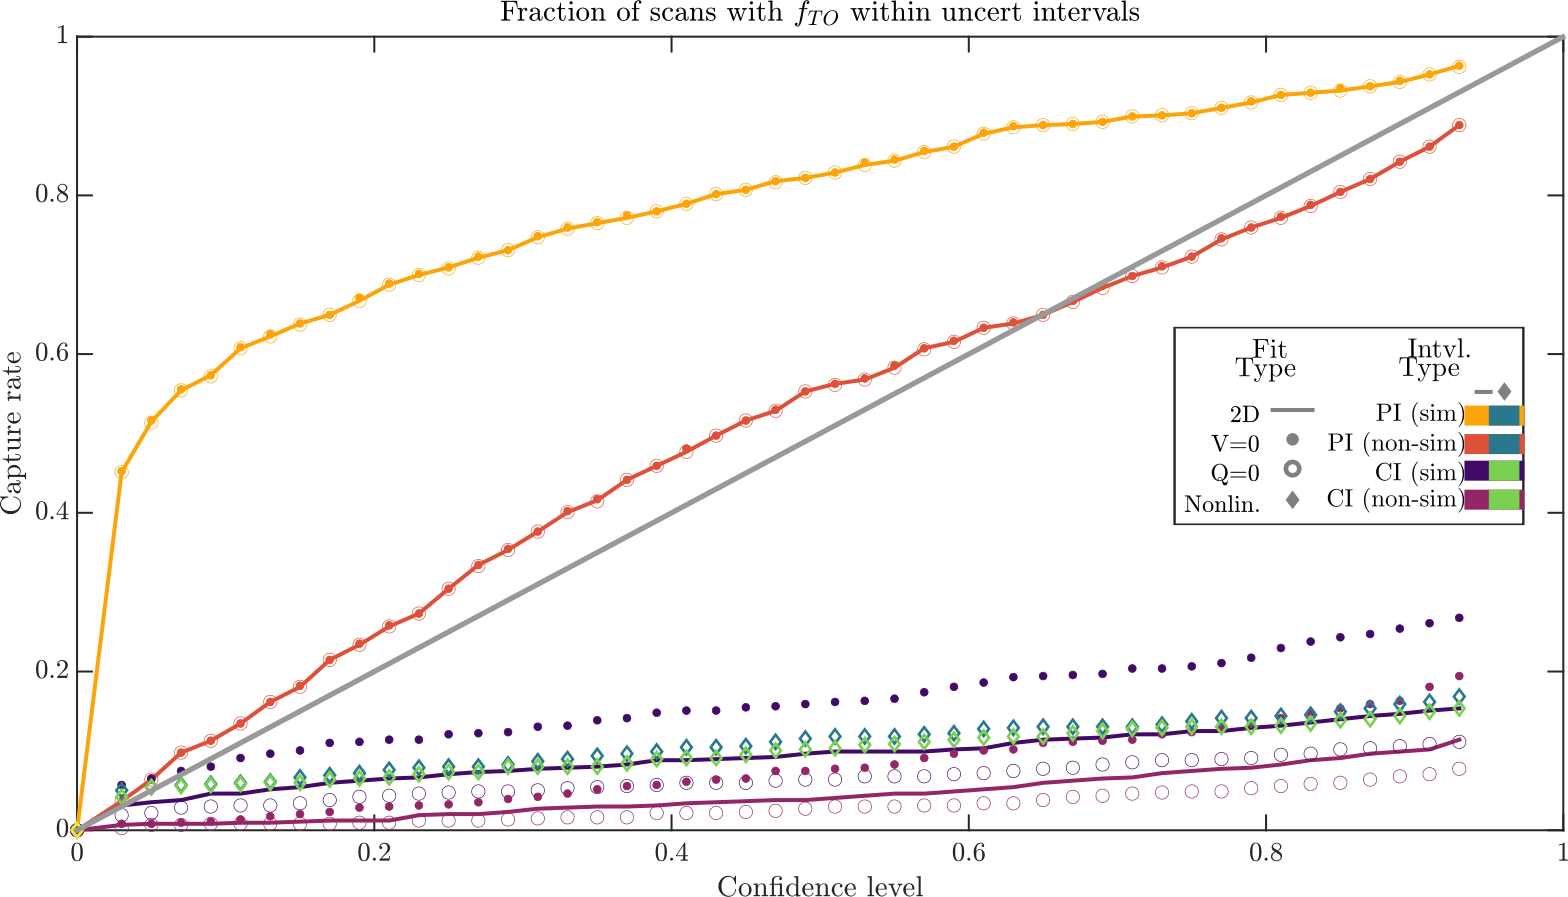
\includegraphics[width=\textwidth]{fig/tuneout/capture_rates}
	% \caption{Distinguishing variance from confidence with prediction bands.}
	% % top data:\(\beta^V \cos(\theta_k)=13240(70)\)~MHz, and \(\beta^T \sin^2(\theta_k)=1140(20)\)~MHz
	% % bottom data: \(\beta^V \cos(\theta_k)=13012(100)\)~MHz, and \(\beta^T \sin^2(\theta_k)=550(100)\)~MHz
	% \label{fig:full_tune_out}
	% \end{figure}


	% It is clear here that the estimated statistical error in the determined TO frequency for each scan is far less than spread between the the model and the data. (factor of 6 between SEWM of combined data and the sd of redisulas, will calc for each unbinned data pt) We attribute this to imperfections in the polarization measurement and variation of the magnetic field pointing.

	% The fit is weighted by the square of the uncertainty in each TO measurement $1/\sigma^2_{f_{TO}}$. The measured TO for each xx shot scan over wavelength for a given polarization is included in the fit as its own data point.
	% The fit is conducted with a global least squares prefitter that is constrained such that $-\pi/4<\theta_k<\pi/4$ and  $\beta^T>0$ which is then fed to an unconstrained fitter. 
	% In this way only a single parameter is required from theory, namely the sign of the tensor polarizability around the TO wavelength. This approach assumes that the tensor and vector polarization is approximately constant about the TO, consistent with theory [REF]\brycecom{from LYT}.

	% the frequency (wavelength) of light at which the atoms experience no perturbation is determined for some input probe polarization state and (ii) many of these measurement's (with varying degrees of circularity and linear orientation) are  combined and fit in Stokes space to determine the TO Scalar Minus Half Tensor (TOSMHT). The analysis for a given polarization state generally consists of hundreds of runs of the experiment grouped together to produce a measured TO for that polarization configuration.

	% and permits us to discern a peak potential energy of as little as 10$^{-35}$J. This is, to our knowledge, the smallest precision in a potential energy measurement reported to date \cite{Henson22}.  


\subsection{Validating linearity against theory}
 
We can use the values of the fit parameters to estimate the size of the polarization-dependent contributions to the measurement. That is, as a sanity check, we can make a low-precision comparison between theoretical predictions for the coefficients $\beta^V$ and $\beta^T$, and also compare the predicted and experimental value of the polarizability gradient $d\alpha/df$. These values are summarized in Tab. \ref{tab:param_compare} and the means by which we estimate them are given below. These values are not the primary interest of this work and accordingly we do not expect precise values to come from the experiment. However, we should expect that the range of values obtained from the experiment should at least include the theoretical prediction. 

%   - beta^V est 15070.4(-601.4,779.4)
%     - Theory val 12200.00
%     - Val ratio 1.24(-0.05,0.06)
%   - beta^T est 2635.0(-688.9,1201.3)
%     - Theory val 3400.00
%     - Val ratio 0.77(-0.20,0.35)


	First, we attend to an estimate of the gradient $d\alpha/df$, starting with its relation to the probe-beam induced shift $\Omega_\textrm{probe}^2$ in the (squared) trapping frequency (c.f. Eqn. \ref{eqn:omega_probe}),
	\begin{align}
	\frac{d~ Re(\alpha)}{d~f}&=A^{-1}\frac{d~\Omega_{\text{probe}}^2}{d~f},~\textrm{where}\\
	    A&=\frac{P}{m \epsilon_{0} c \pi^3  w_0^4}=\frac{1}{ \pi^2 m \epsilon_{0} c }\frac{I}{2 w_0^2}.
	    \label{eqn:da_df}
	\end{align}
	Figure \ref{fig:freq_scan} shows a response with a slope of approximately $d\Omega_\textrm{probe}^2/df \approx 30$ Hz$^2$/GHz, which is typical of the data collection runs. 
	We then need to compute the conversion factor, which in turn demands an estimate of the power and spot size of the laser beam at the interaction zone.
	We recorded of the probe beam power and profile obtained from measurements outside the vacuum chamber, but the vacuum window (through which the beam passes) subtly alters the beam profile and focal point.
	However, the arguments leading to Eqn. (\ref{eqn:omega_probe}) show that the tune-out is independent of the probe beam intensity (to first order) and therefore regular measurements of the beam profile were not necessary. 
	Hence, based on the measurements we did take of the profile through the course of the experiment, we adopt a conservative margin of error for the beam waist, using the range 15(5) $\mu$m. 
	Similarly we assume knowledge of the beam power at the trap to within about 20\%, i.e. $P\approx140(30)$ mW. The conversion factor $A=\frac{P}{m \epsilon_{0} c \pi^3  w_0^4}$ consistent with these values is $A\approx5(7)\times10^{45}$ kg A$^{-2}$  s$^{-6}$. 
	The uncertainty in this estimate is obtained by simple propagation of errors, and is dominated by the strong dependence on the beam waist that converts a 20\% error in $w_0$ into a $\sim140$\% uncertainty in $A$. 
	Note that Eqn. (\ref{eqn:da_df}) shows that the value $A$ must be positive if $d\Omega_{\textrm{Probe}}^2/df$ is positive (which it is in all shots included in the analysis), hence we can specify the uncertainty could be stated more strictly as $A=5^{+7}_{-5}\times10^{45}$.
	However, as this quantity is calculated for the purposes of a sanity-check, this detail is omitted from the remainder of the calculation.
	Thus the experimental value of the polarizability gradient is obtained by $d\Omega_{\textrm{Probe}}^2/df A^{-1}$ and has the value $5(7)\times10^{-54}~\textrm{C}~\textrm{m}^2~\textrm{V}^{-1}~\textrm{Hz}^{-1}$,
	 where the bracketed digit includes the statistical variation across all runs used in the analysis as well as the uncertainty due to imperfect knowledge of the beam parameters at the interrogation zone. 
	This value is included, with associated uncertainty interval, in Tab. \ref{tab:param_compare} and is broadly consistent with the theoretical value in that the theoretical value lies within the margins of error.
	The accuracy of this estimate is fundamentally limited by the quartic dependence on the beam waist, which was not precisely quantified as it is not a critical parameter for the purposes of measuring the tune-out frequency (Eqn. \ref{eqn:omega_probe} shows that the waist must only be stable, not precisely measured, to determine the tune-out frequency). However, as we discuss below in the context of the hyperpolarizability, the error induced by imperfect knowledge of the probe beam intensity is not significant.

	As for the polarization-dependent effects, our nonlinear fitting procedure returns $\beta^T\sin^2(\theta_k)=1140(20)$ MHz but, as noted above, unique values of $\beta^T$ and $\theta_k$ are not obtainable because the physical model is over-articulated (i.e. has more parameters than degrees of freedom due to physical constraints). 
	We can estimate the angle $\theta_k\approx 30^\circ$ from simulations of our magnetic trap, which is consistent with the fitted value of $25^\circ$. 
	Working with an estimate of $\theta_k = 27.5\pm(5)^\circ$, we determine the values shown in Tab. \ref{tab:param_compare}. 
	These calculations indicate effect sizes that are of the same order of magnitude as theoretical predictions, and whose uncertainty bounds also include the predicted value.
	Similarly, the theoretical value for $\beta^V$ is of comparable scale to the experimental value.
	The conclusion of the working in this section is that our linearized model for the tune-out is a good approximation for the system under relevant test conditions because our (approximate) inferences of relevant parameters agree with theoretical expectations.

	\begin{table}
	    \centering
	    \begin{tabular}{l c c c c c}
	        \hline\hline
	         Quantity & $d\alpha/df$ (C m$^2$ V$^{-1}$ Hz$^{-1}$) && $\beta^V$ (MHz) &&  $\beta^T$ (MHz)\\
	         \hline
	         Experiment & $5(7)\times10^{-54}$ &&  $1.5(1)\times10^4$ && $2.6^{+1.2}_{-0.6}\times10^3$\\
	         Theory & $1.78\times10^{-53}$ && $1.22\times10^4$ && $3.4\times10^3$\\
	         Ratio exp./thr. & 0.3(4) && 1.2(1) && \(0.8^{+0.4}_{-0.2}\)\\
	         \hline\hline
	    \end{tabular}
	    \caption{Comparison between the theoretical and experimentally-determined values for the gradient of the polarizability, and the reduced-vector and reduced-tensor polarizabilities. Note that the latter two are coupled via the fit model (through $\theta_k$) and hence this determination is not unique. Nonetheless, these comparisons show that the experimental values are generally consistent with the theoretical predictions. The parentheses denote the 1$\sigma$ uncertainty in the final digit. Uneven uncertainty intervals are quantified by the upper (superscript) and lower (subscript) values. All experimental values are within 2$\sigma$ of the predicted values.}
	    \label{tab:param_compare}
	\end{table}
\section{Systematic effects}
\label{sec:systematic_effects}

	
	

\subsection{Polarization}

	 The extraction of \(\fto(-1,0)\) needs an accurate determination of the probe beam polarization at the point of interaction with the atoms. 
	 As we did not have polarization optics mounted in vacuo, we inferred it from measurements outside the vacuum system. 
	 We estimated the contribution of two effects: the birefringence of the vacuum windows and the variation of polarization across the beam profile.
	 

\subsubsection{Birefringence}
	
	The polarization of the light may be altered as it passes through the final optical element: The glass window into the vacuum chamber.
	This means that the in-vacuum polarization may be different from the polarization set by the pre-insertion optics and measured prior to vacuum entry.
 	We estimated the size of this effect by measuring the probe beam polarization before it entered the vacuum system, and again after it exited through a second window\footnote{A portion of the probe beam escaped back through the in-vacuum mirror at the LVIS and then the insertion window for the horizontal trapping beam of the first MOT, making this possible.}.
 	We determined the error by running the $\fto(-1,0)$ analysis, as above, using both sets of polarization measurements (see Fig.~\ref{fig:full_tune_out}). 
 	We found that these values agreed within \(200\)~MHz, and hence used the average of the two as the final measured value and, and the difference is taken to be the uncertainty associated with the window birefringence. 

\subsubsection{Polarization across the beam}

	We also observed a small variation in the polarization across the transverse profile of the beam, as measured through a 1mm-diameter aperture.
	We determined that the mirrors in the pre-vacuum optics were the culprit.
	We characterized this by measuring polarization at several points across the beam.
	Using the polarization measured far from the beam axis produces a value of \(f_{\mathrm{TO}}(-1,0)\) that is up to \(400\)~MHz different from using the polarization at the beam center. 
	However, these contributions from differently-polarized light are weighted by their respective intensities, and accordingly the  weighted values produce a \(150\)~MHz uncertainty in $\fto$.

\subsection{Linearity} \label{sec:syst.subsec:lin}
	There are two instances in the preceding discussion where a linear approximation has been made in order to render the analysis tractable.
	Here I quantify the possible systematic shifts that could arise from these approximations.

\subsubsection{Linearity of the frequency shift}
	The first instance is the assumption that the perturbation $\Omega_\mathrm{probe}^2$ is linear with respect to the probe beam frequency, which leads to the use of linear regressions on the individual scans to obtain \(f_{\mathrm{TO}}(\st{Q,V})\).
	This is only approximately true: The polarizability is a nonlinear function of laser frequency at larger distances from $\fto$ (on the THz scale). 
	Nonetheless, quadratic (and higher) terms included in the fits to the laser scans were not significant.
	Using a theoretical model of the polarizability, we found that a linear fit spanning 4~GHz either side of the tune-out would return a zero-crossing only $-88(1)$~kHz from the true tune-out. 
	If we were to measure out 40 GHz either side of the tune-out, this shift would increase to $-9.6(2)$~MHz because the quadratic (and higher-order) terms become more significant, reducing the accuracy of the linear fit.
	However, these shifts are reduced to 0.6~kHz and 40~kHz in the 4~GHz and 40~GHz cases, respectively, by including a quadratic term.
	In comparison to the other systematic effects, this linearization introduces a negligible error.

	% Our analysis to obtain \(f_{\mathrm{TO}}(-1,0)\) assumes the perturbation $\Omega_\mathrm{probe}^2$ is linear with respect to the probe beam frequency. 
\subsubsection{Linearity of hybrid potential}
	We also made a linear approximation when deriving the relation $\Omega_{\text{net}}^2=\Omega_{\text{trap}}^2+\Omega_{\text{probe}}^2$, which was derived assuming the probe beam created a harmonic potential, ignoring higher-order derivatives of the Gaussian optical potential.
	The overlapping combination of harmonic traps is also harmonic, thus the equations of motion of an oscillating BEC are given by linear second-order ODEs.
	In contrast, a feature of oscillatory motion in anharmonic potentials is that the period of oscillation depends on the total energy (\emph{i.e.} on the amplitude).
	We checked for this by fitting the damped-sine model to different (contiguous) subsets of the atom laser pulses.
	While we did observe that the largest oscillations were 0.3 Hz slower than the smallest, there was no discernable effect on the zero crossing $\fto$.  
	Hence, again, this was found to be a suitable approximation.


\subsubsection{Linearity in the beam intensity}
	
	We measured \(\Omega_{\mathrm{probe}}\) as a function of probe beam power, with the polarization and frequency fixed, to constrain any shift with respect to probe beam intensity. A second-degree polynomial was sufficient to describe the response, illustrated in Fig.~\ref{fig:probe_beam_linearity}. 
	We deduced that using a linear fit at experimentally-relevant beam powers, rather than a quadratic fit, would lead to a  \(-24(30)\)~MHz change in the determined tune-out.

		\begin{figure}
	    \begin{minipage}{0.58\textwidth}
	    \vspace{0pt}
	    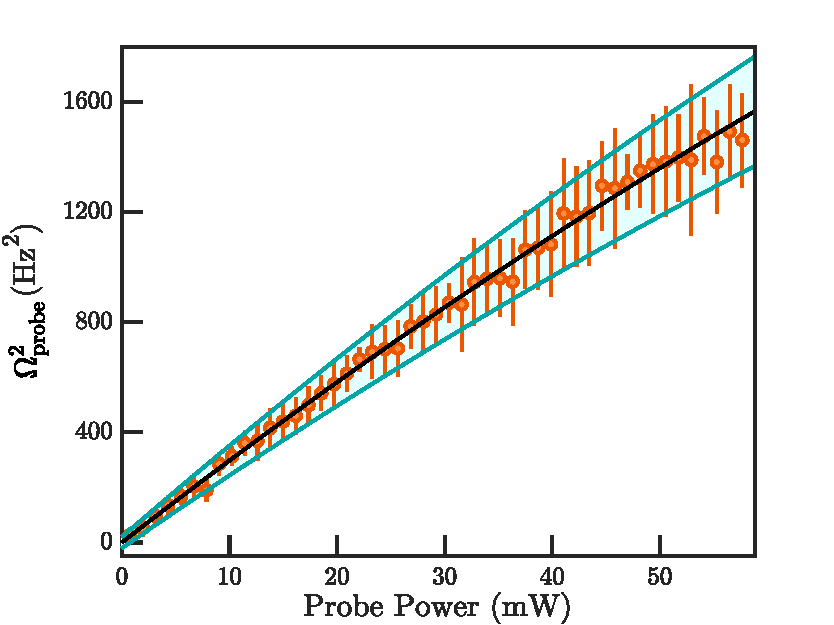
\includegraphics[width=\textwidth]{fig/tuneout/probe_beam_linearity}
	    \end{minipage}
	    \hfill
	    \begin{minipage}{0.4\textwidth}
	    \vspace{0pt}
	    \caption{Testing for nonlinear response versus power. We set the  probe frequency 20~GHz blue of $\fto$,  producing a strong potential, and fit the response against the laser power P with the model \( \Omega_{\mathrm{probe}}^2 = a  P - b P^2 \).  The fit parameters are \(a=\text{30.3(1)}\times 10^{-3}\text{~Hz}^2\text{W}^{-1}\), \(b= \text{0.06(2)} \times 10^{-6}\text{~Hz}^2\text{W}^{-2}\), and $\chi^2$/dof=0.992. Higher-order terms  were not statistically significant. The \(1\sigma\) (observation) confidence interval is shaded. 	    }
	    \label{fig:probe_beam_linearity}
	    \end{minipage}
	\end{figure}



\subsection{Hyperpolarizability}

	The working above also assumes that the metastable-state energy shift due to a nonzero polarizability is a linear function of the light field intensity. 
	We combined theoretical predictions and experimental measurements to obtain an estimate for this error.
	

	\begin{figure}[t]
	    \centering
	    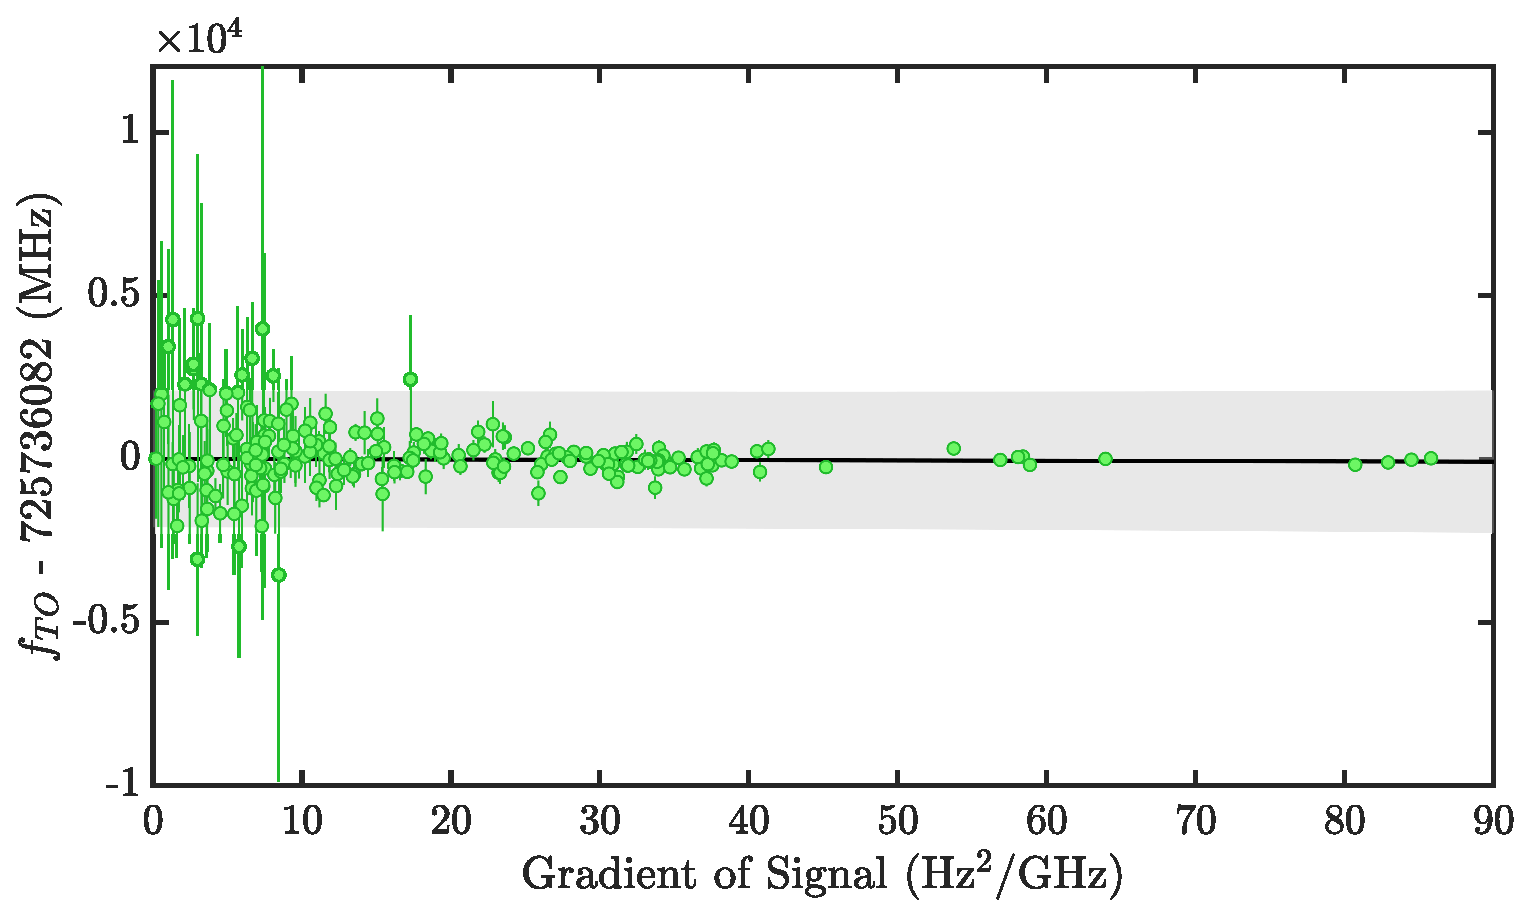
\includegraphics[width=\textwidth]{fig/tuneout/hyperpolz_graph_full}
		\caption{Measured tune-out dependence on probe beam intensity. The highest signal gradient (right) corresponds to a peak light field intensity of \(\sim4\times10^{8}\: \mathrm{W}\cdot \mathrm{m}^{-2}\). Error bars show the variance of binned data. The shaded region indicates the \(1\sigma\) observation interval, quantifying the variance in the data.  An uncertainty-weighted linear fit to the full data set data with parameters offset\(=725\,736\,082(3)\)~MHz and gradient -1(2) MHz/(Hz\(^2\)/GHz) is shown. 95\% confidence intervals in parameters are given in parentheses. This fit has $\chi^2$/dof=0.987 and determines that the gradient dependent tune-out shift is $30(50)$~MHz for the power used in the main measurement, which is statistically consistent with zero.
		    % former grad \(=-1.2(1.5)\)~MHz/(Hz\(^2\)/GHz)
		    }
	    \label{fig:hyperpolarizability}
	\end{figure}

    
\subsubsection{Theoretical treatment}

	The energy of an atom in the presence of an electric field \(E\) oscillating at a frequency \(f\) is 
	\begin{equation}
	\mathcal{E}=\mathcal{E}_0 - \frac{1}{2} \alpha(f) E^2 - \frac{1}{24} \gamma(f) E^4 + \ldots \, , \label{eqn:energy_shift}
	\end{equation}
	where \(\mathcal{E}_0\) is the energy of the unperturbed atom, \(\alpha(f)\) is the dynamic polarizability, and \(\gamma(f)\) is the (second) hyperpolarizability.  
	For a monochromatic light field, the time-averaged electric field amplitude is related to the intensity $I$ via
	\begin{equation}
	    E^2=\frac{2 I}{c \epsilon_0},
	\end{equation}
	where \(c\) is the speed of light and \(\epsilon_0\) is the permittivity of free space. 
	A tune-out measurement may be shifted due to the dynamic polarizability cancelling any contribution from the hyperpolarizability. 
	We can estimate this shift by noting that, by definition, \(\mathcal{E}=\mathcal{E}_0\) at the measured tune-out, and expanding the polarizability to first order about the tune-out.
	Thus Eq.~(\ref{eqn:energy_shift}) gives 
	
	\begin{equation}
	 (f-f_\mathrm{TO} ) = - \frac{1}{12} \gamma(f) \left(\frac{2 I}{c \epsilon_0}\right) \left(1\left/ \frac{\partial\alpha}{\partial f}\bigg|_{f=f_\mathrm{TO}} \right. \right).
	\end{equation}
	From the theoretical calculations, the dynamic hyperpolarizability  is $6.964\times10^{-58}$ $\mathrm{C}^4\mathrm{m}^4\mathrm{J}^{-3}$ (about $-1.12\times10^{7}$ a.u.) at the tune-out. The probe beam intensity in the experiment was less than $10^{9}\: \mathrm{W} \mathrm{m}^{-2}$ and thus a shift due to the hyperpolarizability is  constrained to be below 1.5~MHz, which is dominated by other systematic effects.

	% High precision atomic theory predicts that the dynamic hyperpolarizability at the tune-out is \(6.964\times10^{-58}\: \mathrm{C}^4\mathrm{m}^4\mathrm{J}^{-3}\), which is much larger than prior the prior prediction \(1.2\times10^{-58}\: \mathrm{C}^4\mathrm{m}^4\mathrm{J}^{-3}\) \cite{Grunefeld}/
	% Assuming the larger yields an estimate that the intensity-dependent shift is up to $2\times10^{-3}\: \mathrm{Hz} \mathrm{W}^{-1} \mathrm{m}^2$. 
	% Given the probe beam intensities used in this experiment were  $<10^{9}\: \mathrm{W} \mathrm{m}^{-2}$, the magnitude of this shift is $<1.5$~MHz and thus dominated by other systematic effects.
	% ($-2\times10^{6}$ atomic second hyperpolarizability units).

\subsubsection{Experimental treatment}

	We also constrained the effect of the hyperpolarizability using an independent experimental approach, by studying the effect of the light intensity on the the measured tune-out. 
	The gradient of \(\Omega_{\text{probe}}^2\) with respect to the laser frequency gives an indirect measurement of the intensity in the region of interaction, and the effect of beam power on the tune-out frequency (via this proxy) is shown in Fig.~\ref{fig:hyperpolarizability}.
	We evaluate the linear fit to the data at the experimentally-relevant gradient of $\approx 30$ Hz$^2$/GHz and find that the resulting shift is 30(50) MHz, which is statistically consistent with zero and with the (smaller) estimate made above on theoretical grounds.
	

\subsubsection{DC Electric Field}

	A worst-case estimate of any DC electric field background is $2~\text{kV}\cdot\text{m}^{-1}$. 
	We can use an approach similar to that of the hyperpolarizability  and find a worst-case shift of \(10^{-2}\)~MHz.

\subsection{Broadband Light}
	\begin{figure}
	    \centering
	    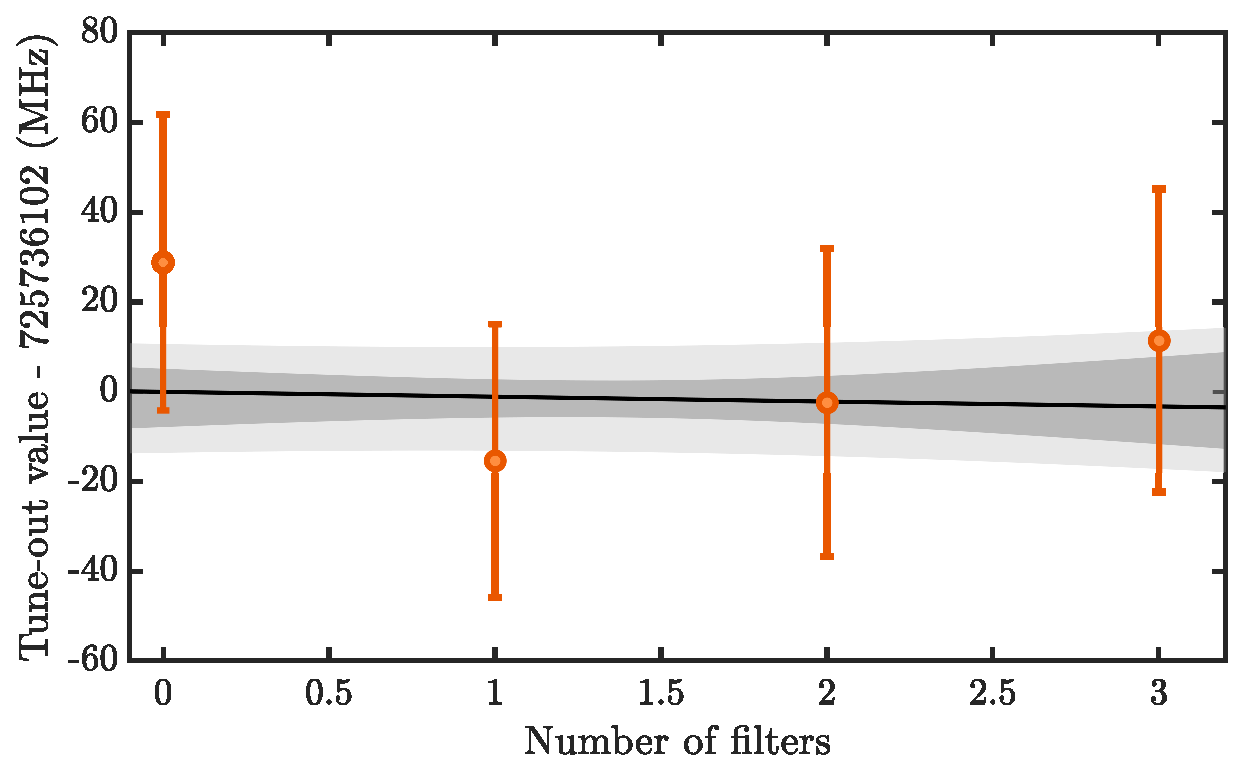
\includegraphics[width=\textwidth]{fig/tuneout/filt_dep_new}
	    \caption{The tune-out frequency as measured with fixed probe beam polarization and power, as a function of the number of filters in the beam path. The gradient of this dependence is -1(5)~MHz/filter, and hence zero within error. The linear fit has $\chi^2$/dof=0.6406. The light region shows the observation interval, and the dark region shows the confidence interval.
	    }
	    \label{fig:broadband light dependence}
	\end{figure}

	Broadband background light could be produced, for example, by  spontaneous emission in the Ti:S laser which is then amplified in the laser cavity. 
	In the presence of weak broadband light, the energy of the atom shifts by the (integrated) pointwise product of the spectral power density and the polarizability. 
	Because the magnitude of the polarizability increases superlinearly with the detuning from the tune-out ($|\alpha(f)| > \alpha'(f) (f-\fto)$ for large detunings), this effect puts a large weight on the tails of the laser line profile $g(f,\Gamma)$ and may shift the apparent tune-out from its actual value by contributing an energy proportional to $\int g(f,\Gamma)\alpha(f)~df$. 
	This places demanding constraints on the tolerable spectral background of the probe laser. 
	This has been a challenge for measurements in other species \cite{HolmgrenThesis}. 
	
	Our use of a frequency doubled laser system provides some protection from this because the doubling cavity suppresses broadband light that might originate in the Ti:S, unless it happens to have a wavelength equal to a multiple of the doubler's free spectral range. 
	Futher suppression is obtained by passing the probe beam through a series of optical filters: a 450~nm shortpass filter (Thorlabs FESH0450, optical density $>5$ between 450~nm and 1200~nm), a 415~nm band-pass filter (Semrock FF01-415/10-25, with a 27~THZ (15.3~nm) FWHM and optical density $>4$ between 250-399~nm and 431-1100~nm), and finally an angle-tunable filter with a 0.9~THz (0.5~nm) FWHM, which we centred on \(\sim 413\)~nm.

	In principle, one could use a spectrometer to measure the spectral power density of the background, but the requisite dynamic range to observe such small effects near a laser peak makes this unfeasible.
	Instead we used a scheme similar the one described in \cite{Leonard15}, and measure the tune-out as a function of the number of (progressively narrowing) filtering stages.
	We can then estimate the shift in the  final measurement. 
	As shown in Fig.~\ref{fig:broadband light dependence},  the measured tune-out frequency is independent of number of filters (within statistical error). 
	Therefore we take the standard deviation between the various filters (\(30\)~MHz)  as the uncertainty associated with the spectral background.
	 

	    % \caption{Measured tune-out frequency for a constant probe beam polarization as a function of the number of filters the probe beam light passes through. We find that the gradient of this dependence is \rev{-1(5) MHz/filter, with a fit $\chi^2$/dof=0.6406}, and hence zero within error.



	\begin{table}
	\centering
	% \begin{ruledtabular}
	\begin{tabular}{l|r|r}
	\hline\hline
	Term              & Value &  Uncertainty \\
	\hline
	Measured Value      & 725\,736\,810             & 40      \\
	Polarization        & & \\
	\, \, - Birefringence & -100                   & 200   \\
	\, \, - Beam Anisotropy & 0                   & 150   \\
	Method Linearity    & 24                   & 30       \\
	Hyperpolarizability           & -30                   & 50   \\
	Broadband Light     & 0                     & 30      \\
	DC Electric field   & 0                     & \(\ll 1\) \\
	Wave-meter          & 0                     & 4    \\
	\hline
	Total               &  725\,736\,700            &  260\\
	\hline\hline
	\end{tabular}
	% \end{ruledtabular}
	\caption{Contributions to measured tune-out frequency with associated systematic uncertainties (MHz). The measured value is found using only polarization data measured after the vacuum chamber. The polarization row gives the average of the tune-out frequencies calculated using polarization data pre and post vacuum chamber relative to the measured value (equivalent to assuming the shift from one window is half of the shift calculated using the measurements after both windows), and the uncertainty is equal to the difference between these values. Note that uncertainties are added in quadrature.}
	\label{tab:results}
	\end{table}
% \subsection{Magnetic Field Pointing}
	
% 	Although we do not need perfect knowledge of the magnetic field orientation to employ the preceding method, the field pointing could drift during the months-long data acquisition period, and thus presents a potential source of systematic error.
% 	To constrain this effect, we simulated the magnetic trap \cite{Dall07_laser} and field stabilization system \cite{Dedman07} used in these experiments \footnote{The source code is available at \cite{mag_trap_simulator}.}.
% 	Such a systematic shift can be divided into two contributions: the short-time variation in field pointing due to an atom's motion within the trap during the interrogation, and any long-term drift due to imperfections in the field control system.
% 	In the trap configurations used in this experiment, the magnetic field at the trap centre subtends a  $5.9 \degree $ angle relative to the long axis of the chamber, with which the probe beam is aligned, and a $0.019 \degree$ angle relative to the horizontal plane. 
% 	Our simulations show that the polar angle of the magnetic pointing varies as $0.019 + 0.88 s \degree$, relative to the $x$ axis, where $s$ is the displacement in m.

	A summary of the systematic shifts is shown in Tab. \ref{tab:results}. 
	The main limiting factor in the accuracy of our value for $\fto$ is  the polarization of the laser light. 


\section{Discussion}
\label{sec:TO_discussion}
	Figure~\ref{fig:contributions} shows a comparison of contributions to the theoretical value of the tune-out and the uncertainties in both the experimental and theoretical determinations.
	The combined theoretical and experimental uncertainties yield a  \(\sigma{\sim} 260\)~MHz precision which is much smaller than the contribution of QED effects (\({\sim} 30 \sigma\)), and thus our measurement validates these calculations.
	The retardation correction to the dipole interaction is slightly larger than the combined uncertainty (\({\sim} 2 \sigma\)), but the contribution of finite nuclear size effects (\(5\)~MHz) are not resolvable at this precision. 
	 
	This is the first measurement with sufficient precision to probe the retardation correction, which is significant as they are typically omitted from calculations of the frequency-dependent polarizability \cite{Drake19, Pachucki19}. 
	Overall, we find a \({\sim} 2.5 \sigma\) difference between experiment and theory, including an estimate of the uncertainty due to terms excluded from the theoretical calculation.  
	Notably, if we ignore the retardation correction (as proposed in Ref.~\cite{Pachucki19} and implemented in tune-out frequency calculations for the first time in this work), then the difference is only \({\sim} 0.5 \sigma\).  
	The retardation contribution could be subject to a more stringent test if the measurement precision could be improved by an order of magnitude (see section \ref{sec:TO_conc} for comments towards this).
	
	\begin{figure}[t]
	    \centering
	    \includegraphics[width=\textwidth]{fig/tuneout/contribution_bar_chart_v7.png}
	    \caption{Theoretical contributions to the tune-out value in comparison to uncertainties in the theoretical and experimental determinations of the \(\TO\) tune-out frequency.}
	    \label{fig:contributions}
	\end{figure}


	
	Using this method we can infer the peak value of the energy shift induced in the atoms by the probe beam. 
	Through Eq.~(\ref{eqn:omega_probe}), a measurement of the shift in trap frequency determines the curvature of peak of the Gaussian optical potential energy surface. 
	Along with knowledge of the beam spot size at the focus, the inferred curvature completely specifies the geometry of the optical potential. 
	We typically achieve an uncertainty in the tune-out of approximately 1.2~$\text{GHz}$ per $\sqrt{N_\text{shots}}$, where \(N_\text{shots}\) refer to the number of BEC's used (including calibration and probe beam measurements). 
	A single scan takes approximately 700~s (12~minutes) and consists of 26 trap frequency measurements (BEC productions). 
	As such, one full scan (26 trap frequency measurements) gives an uncertainty of $\sim 1.2\;\mathrm{GHz}/\sqrt{26}=235$~MHz\footnote{The number of measurements taken to find the tune-out for a given polarization varies from 50 to a few thousand for the data presented here.}.
	Thus, we can indirectly measure the absolute energy shift in the $\MetastableState$ state with a sensitivity of $1.7\cdot10^{-33}\mathrm{J}/\sqrt{\mathrm{sec}}$, where the time is the probe beam interrogation time. 
	In the case of the measurement with the lowest frequency uncertainty in $f_\textrm{TO}$, (30~MHz), the minimum potential energy peak we can thus discern is approximately $10^{-35}\mathrm{J}$ ($U/k_B=3$~pK).

\subsection{Improvements upon past measurements}

	The past measurement of this tune-out frequency \cite{Henson15} obtained a 4 GHz uncertainty in the determined value of $\fto = 725.7249$ THz, thus the 263 MHz uncertainty presented here amounts to a 15-fold improvement in precision (note that here the statistical and systematic errors for each measurement are combined in quadrature for ease of comparison).
	There are four factors underlying the improved result.
	\begin{enumerate}
		\item \textbf{Laser power:} The present measurement applied a 150 mW probe beam at the point of vacuum entry, whereas the original measurement used a 3 mW laser diode (subject also to losses when passing through the focusing optics). 
		\item \textbf{Characterisation of polarization effects:} As described below (section \label{sec:polz_dep}, especially Eqn. \ref{eqn:fto_stokes_eqn}), the atomic tune-out point depends quite strongly on the polarization of the electric field with respect to the atom's quantization axis. Accordingly, considerable attention is paid in this chapter to measuring this dependence in order to obtain a single measured value for comparison with theoretical calculations. In contrast, the previous measurement used only linearly-polarized light. The direction of polarization relative to the atomic quantization axis in that experiment is not known. 
		\item \textbf{Probe wavelength precision}: The High Finesse WS-8 wavemeter, obtained especially for this measurement, affords a locking of the probe beam with $\approx$175-fold greater accuracy. Moreover, the day-to-day drift of the wavemeter in the previous measurement was up to 350 MHz \cite{HensonHonsThesis}, larger than the drifts relevant to the present measurement by a similar factor. 
		\item \textbf{Trap frequency determination:} This is the most critical innovation over the past measurement. Previously, the trap frequency was measured by modulating the net trapping potential with a probe beam and using a `lock-in' technique \cite{HensonHonsThesis} based on Fourier analysis of the outcoupling signal of a continuous atom laser. The idea is that the outcoupling efficiency would be modulated at the probe beam modulation frequency, and the phasor response of would cross zero amplitude (with a phase flip) at the tune-out point. However, this signal exhibited a very high variance therefore contributed considerable uncertainty to the final linear fit to determine the tuneout. In contrast, the method employed in this work provides trap frequency measurement accurate to a few dozen ppm \cite{Henson22_PAL}, drastically improving the accuracy of $\fto$ as determined by the fitting procedures defined below.
	\end{enumerate}


\subsection{Comparison With Previous Oscillator Strength Ratio Measurements}
	
	We can extend the approach taken in Ref. \cite{Mitroy13} to a three-level atom (c.f. section \ref{sec:TO_points}) and write the polarizability of an atom in the state $\ket{1}$ as 
	\begin{equation}
	\alpha_1(f) = \frac{f_{12}}{E_{21}^2-h^2 f^2}+\frac{f_{13}}{E_{31}^2-h^2 f^2}
	\end{equation}
	where $f_{12}$ and $f_{13}$ are the oscillator strengths, $E_{12}$ and $E_{13}$ are the excitation energies of the dominant transitions, $f$ is the photon frequency, and \(h\) is Planck's constant. 

	The condition $\alpha(\fto)=0$ implies that
	\begin{equation}
		 \frac{f_{12}}{E_{21}^2-h^2 \fto^2} = -\frac{f_{13}}{E_{31}^2-h^2 \fto^2},
	\end{equation}
	and hence
	\begin{equation}
		\frac{f_{13}^2}{f_{12}^2} = \left(\frac{E_{31}^2-h^2 \fto^2}{E_{21}^2-h^2 \fto^2}\right)^2.
	\end{equation}

	The fractional sensitivity of the ratio $X=\frac{f_{13}^2}{f_{12}^2}$ to the tune-out is
	\begin{align}
	    \frac{\delta X}{X} &= \frac{1}{X} \cdot  \frac{\partial X} {\partial f_{TO}} \delta f_{TO} \\
				    &=\frac{2  h^2 f_{TO} (E_{12}^2-E_{13}^2)}{(E_{12}^2-h^2 f_{TO}^2) (-E_{13}^2 + h^2 f_{TO}^2 )} \cdot \delta  f_{TO}\\
				    & = \frac{-2 f_{TO}^2 (f_1^2-f_2^2)}{(f_1^2-f_{TO}^2)(f_2^2-f_{TO}^2)} \frac{\delta  f_{TO}}{f_{TO}}
	\end{align}
	where $f_i=E_{1i}/h$.
	Given the dominant transition manifolds at 276.7465 THz (\(\MetastableState \to \TOUpperStateManifold \)) and 770.7298 THz (\(\MetastableState \to \TOLowerStateManifold\)), as well as our value for the tune-out frequency of \(f_{TO}=725.73670\) THz, we reach a fractional uncertainty in the oscillator strength ratio of 6~ppm.
	We can compare our measurement to others in the literature by using frequency of the dominant transitions and the measured tune-out value to estimate the sensitivity to the ratio of transition strengths. 
	We find that our measurement improves against the previous record of 15~ppm, reported in Ref.~\cite{Leonard15}. 
	We note that the relative uncertainty in $X$ equals the relative uncertainty in the ratio of transition matrix elements, which were the quantity calculated in Ref.~\cite{Leonard15}.
	We further note that this method is approximate and neglects the contribution from the DC polarizability, however this is a small effect and not needed for such coarse comparison of sensitivity. 
	Thus, we claim that our measurement of the $\TO$ tune-out wavelength produces the most precise constraint of relative transition rates in any atomic system to date. 


\subsection{Conclusion}
	\label{sec:TO_conc}
	Our experimental determination of 725\,736\,700\,$(40_{\mathrm{stat}},260_{\mathrm{syst}})$ MHz has a relative precision of $4\times 10^{-7}$, constituting the most precise measurement of atomic transition rate ratios to date \cite{Mitroy13}, and is 2.5$\sigma$ larger than the theoretical prediction. 
	This measurement determines the ratio of oscillator strengths to 6 ppm, which is a factor of two improvement on the previous record. 
	Furthermore, our novel method for measuring the dipole potential is able to discern a peak potential energy of as little as 10$^{-35}$ J . This is, to our knowledge, the highest precision in a potential energy measurement reported to date \cite{Henson22}.
	 
	In future precision measurements of tune-out points, significant improvements would follow from more precise calibration of the light polarization.
	One solution would be to use in-vacuum optics and make finer measurements of the angle of the beam axis relative to the magnetic field.
	These improvements would allow for independent tests of the scalar, vector, and tensor polarizabilities, thus yielding more information about the structure of the helium atom and QED itself.

	The method above could be used to measure other tune-out frequencies in helium or other species.
	It could also serve as a means to investigate other issues relating to QED. 
	If a future measurement could be made with MHz-level precision,  this tune-out could be used to calculate the nuclear charge radius of helium. 
	Thus this method, and its future improvements, may continue to  clarify the `jewel of physics.'

\vfill


\begin{flushright}
\singlespacing
{\emph{
``Imagination reaches out repeatedly trying to achieve some \\
higher level of understanding, until suddenly I find myself \\
momentarily alone before one new corner of nature’s \\
pattern of beauty and true majesty revealed. \\
That was my reward."}\\ 
- Richard P Feynman\footnote{Nobel banquet speech, 1965}}
\end{flushright}
\onehalfspacing




% \section{Note stash}



% \subsubsection*{Calculation of \(C\) and \(D\)}
% 	Consider light propagating along the \(z-\)axis (\textit{i.e.} light vector \(\vec{k} = \left(0,0,1\right)\)), the Jone's vector of this light is given by:
% 	\begin{align}
% 	    \vec{u} &= \begin{pmatrix}
% 	    u_{0,x} \\
% 	    u_{0,y} e^{i \phi_y} \\
% 	    0
% 	\end{pmatrix}.
% 	\end{align}
% 	By definition the stokes parameters are defined as follows (in order from first to fourth):
% 	\begin{align}
% 	    \mathcal{I} &= |u_x|^2 + |u_y|^2 \\ 
% 	    \mathcal{Q} &= |u_x|^2 - |u_y|^2 \\
% 	    \mathcal{U} &= 2 \text{Re} \left(u_x u_y^*\right) \\
% 	    \mathcal{V} &= -2 \text{Im}\left(u_x u_y^*\right)
% 	\end{align}
% 	where \(\vec{u} = (u_x,u_y,u_z)\). Note we only wish to consider that normalised Jones vector/ Stokes parameters, hence \(\mathcal{I}=1=u_{0,x}^2+u_{0,y}^2\). Let the plane formed by the light vector \(\vec{k}\) and the magnetic field vector at the atoms (the quantization axis) \(\vec{b}\) be the \(y-z\) plane, hence if the angle between the light vector and the magnetic field is \(\theta_k\) then:
% 	\begin{align}
% 	        \vec{b} &= \begin{pmatrix}
% 	    0 \\
% 	    \sin(\theta_k) \\
% 	    \cos(\theta_k)
% 	\end{pmatrix}.
% 	\end{align}
% 	Now if the polarisation is rotated by an angle \(\theta_\varepsilon\) the Jone's vector becomes 
% 	\begin{align}
% 	    \vec{u} &= \begin{pmatrix}
% 	    \cos(\theta_\varepsilon) u_{0,x} -\sin(\theta_\varepsilon) u_{0,y} e^{i \phi_y}\\
% 	    \sin(\theta_\varepsilon) u_{0,x} +\cos(\theta_\varepsilon) u_{0,y} e^{i \phi_y} \\
% 	    0
% 	\end{pmatrix}.
% 	\end{align}
% 	Now to align with equations \ref{eqn:C} and \ref{eqn:D} we want to rotate the axes such that the B-field is pointing along the \(z\)-axis, this corresponds to a rotation matrix of:
% 	\begin{align}
% 	    R_k &= \begin{pmatrix}
% 	 1& 0 & 0 \\
% 	 0 & \cos(\theta_k) & -\sin(\theta_k) \\
% 	 0 & \sin(\theta_k) & \cos(\theta_k)
% 	\end{pmatrix}.
% 	\end{align}
% 	applying this we get the Jone's vector in the B-field's frame of reference (denoted \(\vec{u}'= R_k \vec{u}\) as
% 	\begin{align}
% 	    \vec{u}' &= \begin{pmatrix}
% 	    \cos(\theta_\varepsilon) u_{0,x} -\sin(\theta_\varepsilon) u_{0,y} e^{i \phi_y}\\
% 	    \cos(\theta_k) \left[\sin(\theta_\varepsilon) u_{0,x} +\cos(\theta_\varepsilon) u_{0,y} e^{i \phi_y}\right] \\
% 	    \sin(\theta_k) \left[\sin(\theta_\varepsilon) u_{0,x} +\cos(\theta_\varepsilon) u_{0,y} e^{i \phi_y}\right] 
% 	\end{pmatrix}.\label{eqn:Jones_mag}
% 	\end{align}
% 	Note that in this notation equations \ref{eqn:C} and \ref{eqn:D} are
% 	\begin{align}
% 	    C &= 2 \text{Im}({u'_x}^* u'_y),\\
% 	    D &= 3|u'_z|^2 -1
% 	\end{align}
% 	as they have the B-field along the \(z\)-axis. Combining this with equation \ref{eqn:Jones_mag} we obtain
% 	\begin{align}
% 	    C&=2\cos(\theta_k)\text{Im}\left(\cos(\theta_\varepsilon)^2 u_{0,x} u_{0,y} e^{i \phi_y} -\sin(\theta_\varepsilon)^2 u_{0,x} u_{0,y} e^{-i \phi_y}\right)\\
% 	    &= 2\cos(\theta_k)\text{Im}\left(u_{0,x} u_{0,y} e^{i \phi_y}\right)\\
% 	    &= \cos(\theta_k)2\text{Im}\left(u_x^* u_y\right)\\
% 	    &= -cos(\theta_k) \mathcal{V}\\
% 	    D&=3\sin(\theta_k)^2 \left[\sin(\theta_\varepsilon)^2 u_{0,x}^2 +\cos(\theta_\varepsilon)^2 u_{0,y}^2 + 2\sin(\theta_\varepsilon)\cos(\theta_\varepsilon)u_{0,x}u_{0,y} \cos(\phi_y)\right] -1\\
% 	    \begin{split}&=\frac{3}{2}\sin(\theta_k)^2 \large[\sin(\theta_\varepsilon)^2 u_{0,x}^2 + (1-\cos(\theta_\varepsilon)^2) u_{0,x}^2 +\cos(\theta_\varepsilon)^2 u_{0,y}^2+\\&\quad\quad\quad(1-\sin(\theta_\varepsilon)^2) u_{0,y}^2 + 4\sin(\theta_\varepsilon)\cos(\theta_\varepsilon)u_{0,x}u_{0,y} \cos(\phi_y)\large]-1\end{split}\\
% 	    \begin{split}&= \frac{3}{2}\sin(\theta_k)^2 \large[-(\cos(\theta_\varepsilon)^2 u_{0,x}^2-2\sin(\theta_\varepsilon)\cos(\theta_\varepsilon)u_{0,x}u_{0,y} \cos(\phi_y)+ \sin(\theta_\varepsilon)^2 u_{0,y}^2) \\&\quad \quad + (\sin(\theta_\varepsilon)^2 u_{0,x}^2 + 2\sin(\theta_\varepsilon)\cos(\theta_\varepsilon)u_{0,x}u_{0,y} \cos(\phi_y) + \cos(\theta_\varepsilon)^2 u_{0,y}^2) + u_{0,x}^2 + u_{0,y}^2 \large]-1\end{split}\\
% 	    &=\frac{3}{2}\sin(\theta_k)^2 \left[-|u_x|^2 + |u_y|^2 + 1 \right] - 1\\
% 	    &=3 \sin^2\left( \theta_k \right) \left(\frac{1}{2} -  \frac{\mathcal{Q}}{2}\right) -1 
% 	\end{align}
% 	where we have used the fact that we are using the normalised Jones vector, hence \(u_{0,x}^2 + u_{0,y}^2 = 1\). 

% 	Consider the polarisation ellipse (the ellipse that the electric field traces out) see figure \ref{fig:ellipse}. Using the ellipse notation we can write
% 	\begin{align}
% 	    \mathcal{Q} &= \cos(2\psi) \cos(2\chi)\\
% 	    \mathcal{V} &= \sin(2\chi)
% 	\end{align}
% 	Next note that the power of a light field is proportional to its electric field amplitude squared so \(p_{min} \propto b^2\) and \(p_{max} \propto a^2\), where \(p_{min}\) and \(p_{max}\) are the minimum and maximum power transmitted through a linear polariser respectively. By trig laws we have 
% 	\begin{align}
% 	\cos(2\chi)&=\cos(\chi)^2-2\sin(\chi)^2\\
% 	&= \left(\frac{a}{\sqrt{a^2+b^2}}\right)^2 - \left(\frac{b}{\sqrt{a^2+b^2}}\right)^2 \\
% 	&= \frac{a^2-b^2}{a^2+b^2}\\
% 	\Rightarrow \mathcal{Q}&=\frac{p_{max}-p_{min}}{p_{max}+p_{min}} \cos(2\theta_\varepsilon)\\
% 	\sin(2\chi) &= 2\sin(\chi)\cos(\chi)\\
% 	&=2 \frac{a}{\sqrt{a^2+b^2}} \frac{b}{\sqrt{a^2+b^2}}\\
% 	&=\frac{2ab}{a^2+b^2}\\
% 	\Rightarrow |\mathcal{V}| &= \frac{2\sqrt{p_{min}p_{max}}}{p_{min}+p_{max}}
% 	\end{align}


	


 
 %Table here

% \subsubsection{Polarization in the Atomic Reference Frame}

% 	\subsubsection{Simplified Explanation}

% 	It can be helpful to consider this process for a simplified system with only linear polarization. In this case the measured tune-out will depend sinusoidally on the angle of the input polarization (\(\theta_{\mathcal{L}}\)). The above method is equivalent to using a sinusoidal fit in order to extract the maximum tune-out value in this dependence, corresponding to the \(f_{\mathrm{TO}}(-1,0)\). The choice of taking the maximum is equivalent to constraining \( \beta^T \). The above method is a natural extension of this simplified approach to also account for the circular component of the light field.


% Magnetic field

% Thermal Hyperpolarizability Shift

% Mean Field

% \hline
% \multicolumn{3}{c}{Theory}\\
% \hline
% Hyp. Polz           & $< 1.5$                   & 0.5     \\
% Magnetic field      & $< 2$                     & 0.01     \\
% DC Stark Shift      & $\ll 1$                   & 0.1    \\
% Thermal Hyperpolarizability Shift & $\ll 1$     & 0.1     \\
% Mean Field          & $\ll 1$                   & 0.1   \\






% 	To estimate the polarization we set up a Rochon prism after the beam exited the vacuum chamber through the LVIS hole and calculated the circularity of the light.




% \subsubsection{Alignment of probe beam}

% 	Alignment We employed three stages of successively increasing precision
% 	to align the probe beam with the magnetic trap, using a 2W? 532nm laser,
% 	followed by a 300mW 450nm beam, and finally using the tunable laser at
% 	approx 405nm?.
% 		The first beam was used for coarse alignment by scanning
% 	the vertical position of the focusing lens and dropping the BEC onto the
% 	phosphor detector.
% 		This technique has been used previously to align
% 	beams - reason being that the repulsive dipole potential of the 532nm
% 	beam creates a fissure in the BEC as the fallinc condensate diffracts
% 	around the beam.
% 		The effect is weak but visible as a dark stripe through
% 	the BEC - at least, ideally.
% 		Sadly, our ingenuity held us back (yet
% 	again).
% 		We used a pickoff plate - a large spherical optic which is
% 	weakly reflective at the target wavelength - for initial scans,
% 	deflecting a fraction of the beam onto a CCD (as described in the Laser
% 	System chapter).
% 		Unfortunately, Bryce dropped this optic at point point
% 	and the rim of the glass lost a chip.
% 		We did not notice for quite some
% 	time that this had altered the strain distribution on the transmitting
% 	surface of the optic, and actually completely destroyed the beam
% 	profile.
% 		How did we find this out, again? This led us to replace the
% 	optic with a mirror on a hinged mount, so we could remove the mirror and
% 	return it to a controllable position.
% 		Once we removed the damaged optic,
% 	we were quite quickly able to find a signal in the disturbed BEC.
% 		I
% 	think we eventually used the atom laser for a better visible signal -
% 	although the phosphor had a better dynamic range, the brightness
% 	difference was hard to see by eye, but integrating over several PALs
% 	gave us a density profile we could use.
% 		We aligned the beam with the
% 	fall path of the condensate by ensuring the destruction was in the
% 	centre of the falling condensate, and then raising the beam step by step
% 	until the signal vanished.
% 		At this point we figured we'd overshot the
% 	trap, so stepped back down and changed to another beam after marking
% 	beam position on the CCD.
% 		We then changed to the high power 450nm beam
% 	because it would produce a strong polarization response in the condensed
% 	atoms.
% 		We then ran successive trap frequency measurements while
% 	adjusting the beam position, looking for disturbances in the oscillation
% 	frequency under the same mechanism by which our measurement method
% 	works.
% 		When this signal reached a maximum with respect to position, we
% 	iterated adjustments in lens position along the beam axis with
% 	adjustments in pointing (as imperfectly aligned optics would couple
% 	these degrees of freedom).
% 		When this signal was maximized, we switched
% 	to the probe beam at 405nm.
% 		At this wavelength the atomic polarizability
% 	is positive so the beam is attractive.
% 		We therefore adjusted the
% 	sequence by switching off the beam at XXX ms after the trap release.
% 	When the beam was aligned we observed a second peak in the detection
% 	rate (picture), from the release of atoms trapped in the beam.
% 		We
% 	iterated this alignment procedure until the number of trapped atoms
% 	saturated - assuming this to be pointing at the BEC.
% 		Then we switched to
% 	alternating shots measuring the trap frequency, as in our measurement
% 	method, and adjusted the lens configuration until the frequency
% 	difference between the measurement and reference shots reached a
% 	maximum.
% 		Then, because the optical dispersion would be such that the
% 	beam pointing and focus would vary with wavelength, we repeated this
% 	procedure after taking steps of a few nm at a time towards the tuneout
% 	wavelength, eventually settling within a few MHz of the transition on
% 	the assumption that a few ppb change in frequency wouldn't bother us.
% 		We
% 	measured the distance from the focus lens to the chamber centre with
% 	reference to a technical diagram, and positioned the CCD at this
% 	distance away from the focus lens (including the reflection off the
% 	alignment mirror) but of course the beam before the focus lens would not
% 	have been perfectly collimated which might have affected the outcome.



	% The gradient of the line was found to vary, and in some cases invert in sign.
	% 	While initially puzzling, this turned out to be a useful validation of the trap frequency picture came from the inadvertent observation of a change of sign of the trap frequency change.
	% 	This was eventually ascribed to the sign change in the second derivative of a Gaussian function, which shows that the small-amplitude oscillation picture described above is actually quite accurate despite all the approximations (like, how big is the BEC?).
	% 	(PIC)